\documentclass[12pt,a4paper]{report}

\usepackage{styles/dolgozat}

\usepackage{listings}
\usepackage{styles/cpp}
\usepackage{styles/python}
\usepackage{styles/java}

\usepackage{hyperref}

\usepackage{float}

\begin{document}
	
	\pagestyle{empty} %a címlapon ne legyen semmi=empty, azaz nincs fejléc és lábléc

% A Miskolci Egyetem címere
{\large
\begin{center}
\vglue 1truecm
\textbf{\huge\textsc{Szakdolgozat}}\\
\vglue 1truecm

\includegraphics[width=4.8truecm, height=4truecm]{images/me_logo.png}\\
\textbf{\textsc{Miskolci Egyetem}}
\end{center}}

\vglue 1.5truecm %függõleges helykihagyás

% A szakdolgozat címe, akár több sorban is
{\LARGE
\begin{center}
\textbf{A szakdolgozat címe}
\end{center}}

\vspace*{2.5truecm}
% A hallgató neve, évfolyam, szak(ok), a konzulens(ek) neve
{\large
\begin{center}
\begin{tabular}{c}
\textbf{Készítette:}\\
Szakdolgozó Neve\\
Programtervező informatikus
\end{tabular}
\end{center}
\begin{center}
\begin{tabular}{c}
\textbf{Témavezető:}\\
Témavezető neve
\end{tabular}
\end{center}}
\vfill
% Keltezés: Hely, év
{\large
\begin{center}
\textbf{\textsc{Miskolc, 2020}}
\end{center}}

\newpage

	
	\newpage
	
	\pagestyle{empty}
	
	%Feladatkiiras
\begin{flushleft}
\textsc{\bfseries Miskolci Egyetem}\\
Gépészmérnöki és Informatikai Kar\\
Alkalmazott Matematikai Intézeti Tanszék\hspace*{4cm}\hfil \textbf{Szám:}
\end{flushleft}
\vskip 0.5cm
\begin{center}
\large\textsc{\bfseries Szakdolgozat Feladat}
\end{center}
\vskip 0.5cm
Nemcsik Dániel (I3I4BP) programtervező informatikus jelölt részére.\newline

\noindent\textbf{A szakdolgozat tárgyköre:} személyes információszervezés, titkosítás\newline

\noindent\textbf{A szakdolgozat címe:} A személyes információszervezés biztonságtechnikai aspektusai\newline

\noindent\textbf{A feladat részletezése:}

\medskip

\emph{A személyes információszervezés (Personal Information Management) az egy személyhez köthető információk (például naptárbejegyzések, kontakt listák, jelszavak) kezelésével foglalkozik. 
\\A dolgozat ennek biztonságtechnikai vonatkozásával foglalkozik. Megvizsgálja, hogy az aktuális, személyenként is több gépes környezetben milyen lehetőségek vannak az adatok szinkronizálására és védelmére. 
\\Bemutatja egy Java asztali alkalmazás elkészítését, amely segíti a felhasználót, hogy az adataihoz az általa használt eszközökön biztonságosan hozzá tudjon férni.}

\medskip

\vfill

\noindent\textbf{Témavezető:} Piller Imre (Tanársegéd) \newline

% \noindent\textbf{Konzulens(ek):} (akkor kötelezõ, ha a témavezetõ nem valamelyik matematikai tanszékrõl való; de persze lehet egyébként is)\newline

\noindent\textbf{A feladat kiadásának ideje:} 2021. szeptember 28.\newline

%\noindent\textbf{A feladat beadásának határideje:}

\vskip 2cm

\hbox to \hsize{\hfil{\hbox to 6cm {\dotfill}\hbox to 1cm{}}}

\hbox to \hsize{\hfil\hbox to 3cm {szakfelelős}\hbox to 2cm{}}

\newpage

\vspace*{1cm}  
\begin{center}
\large\textsc{\bfseries Eredetiségi Nyilatkozat}
\end{center}
\vspace*{2cm}  

Alulírott \textbf{Nemcsik Dániel}; Neptun-kód: \texttt{I3I4BP} a Miskolci Egyetem Gépészmérnöki és Informatikai Karának végzős Programtervező informatikus szakos hallgatója ezennel büntetőjogi és fegyelmi felelősségem tudatában nyilatkozom és aláírásommal igazolom, hogy \textit{A személyes információszervezés biztonságtechnikai aspektusai}
című szakdolgozatom saját, önálló munkám; az abban hivatkozott szakirodalom
felhasználása a forráskezelés szabályai szerint történt.\\

Tudomásul veszem, hogy szakdolgozat esetén plágiumnak számít:
\begin{itemize}
\item szószerinti idézet közlése idézőjel és hivatkozás megjelölése nélkül;
\item tartalmi idézet hivatkozás megjelölése nélkül;
\item más publikált gondolatainak saját gondolatként való feltüntetése.
\end{itemize}

Alulírott kijelentem, hogy a plágium fogalmát megismertem, és tudomásul veszem, hogy
plágium esetén szakdolgozatom visszautasításra kerül.

\vspace*{3cm}

\noindent Miskolc, \hbox to 2cm{\dotfill} .év \hbox to 2cm{\dotfill} .hó \hbox to 2cm{\dotfill} .nap

\vspace*{3cm}

\hspace*{8cm}\begin{tabular}{c}
\hbox to 6cm{\dotfill}\\
Hallgató
\end{tabular}



\newpage

\noindent 1.

\begin{tabular}{cl}
&szükséges (módosítás külön lapon) \\
A szakdolgozat feladat módosítása& \\
& nem szükséges\\
&\\
\hbox to 4cm{\dotfill}&\multicolumn{1}{c}{\hbox to 5cm{\dotfill}}\\
dátum& \multicolumn{1}{c}{témavezető(k)}
\end{tabular}
\vskip1.5mm

\noindent 2. A feladat kidolgozását ellenőriztem:

\vskip1.5mm

\begin{tabular}{l@{\hspace*{4cm}}l}
témavezető (dátum, aláírás):& konzulens (dátum, aláírás):\\
\dotfill&\dotfill\\
\dotfill&\dotfill\\
\dotfill&\dotfill
\end{tabular}

\vskip1.5mm

\noindent 3. A szakdolgozat beadható:

\vskip1.5mm

\begin{tabular}{@{\hspace*{1.3cm}}c@{\hspace*{2.1cm}}c}
\hbox to 4cm{\dotfill}&\multicolumn{1}{c}{\hbox to 5cm{\dotfill}}\\
dátum& \multicolumn{1}{c}{témavezető(k)}
\end{tabular}

\vskip1.5mm

\noindent 4.
\begin{tabular}[t]{@{}l@{\hspace*{1mm}}l@{\hspace*{1mm}}l@{}}
A szakdolgozat& \hbox to 3.5cm{\dotfill} &szövegoldalt\\
              & \hbox to 3.5cm{\dotfill} &program protokollt (listát, felhasználói leírást)\\
              &\hbox to 3.5cm{\dotfill}   &elektronikus adathordozót (részletezve)\\
              &\hbox to 3.5cm{\dotfill} & \\
              &\hbox to 3.5cm{\dotfill} &egyéb mellékletet (részletezve)\\
              &\hbox to 3.5cm{\dotfill} &\\
\end{tabular}
\newline tartalmaz.

\vskip1.5mm

\begin{tabular}{@{\hspace*{1.3cm}}c@{\hspace*{2.1cm}}c}
\hbox to 4cm{\dotfill}&\multicolumn{1}{c}{\hbox to 5cm{\dotfill}}\\
dátum& \multicolumn{1}{c}{témavezető(k)}
\end{tabular}

\noindent 5.

\begin{tabular}{ll}
&bocsátható\\
A szakdolgozat bírálatra& \\
& nem bocsátható\\
\end{tabular}

\vskip1.5mm

\noindent A bíráló neve: \hbox to 8cm{\dotfill}

\vskip4mm

\begin{tabular}{@{\hspace*{1.3cm}}c@{\hspace*{2.1cm}}c}
\hbox to 4cm{\dotfill}&\multicolumn{1}{c}{\hbox to 5cm{\dotfill}}\\
dátum& \multicolumn{1}{c}{szakfelelős}
\end{tabular}

\noindent 6.
\begin{tabular}[t]{@{}l@{\hspace*{1mm}}l@{\hspace*{1mm}}l@{}}
A szakdolgozat osztályzata& &\\
&a témavezető javaslata:& \hbox to 3cm{\dotfill}\\
&a bíráló javaslata:& \hbox to 3cm{\dotfill}\\
&a szakdolgozat végleges eredménye:& \hbox to 3cm{\dotfill}
\end{tabular}

\vspace*{4mm}

\noindent Miskolc, \hbox to 4.5cm{\dotfill} \hspace*{2.5cm}
\begin{tabular}[t]{cc}
\hbox to 6cm{\dotfill}\\
a Záróvizsga Bizottság Elnöke
\end{tabular}

	
	\cleardoublepage
	\pagenumbering{gobble}
	\tableofcontents
	\cleardoublepage
	\pagenumbering{arabic}
	
	\newpage
	
	\pagestyle{fancy}
	
	\Chapter{Bevezetés}

A dolgozat fő célja egy Java asztali alkalmazás elkészítése volt, ami képes többgépes környezetben is biztonságosan eltárolni a felhasználó adatait és visszaadni azokat szinkronizált módon az eszközök között.

A program készítése során különböző problémákat kellett megoldanom, mint például a megfelelő titkosítási algoritmus kiválasztása, adatszinkronizáció elérése különböző eszközök között, esztétikus Java grafikus felhasználói felület létrehozása.

A szakdolgozat a felmerülő problémák potenciális megoldási lehetőségeit és elméleti hátterét mutatja be.

Megpróbálja részletesen ismertetni az adattitkosítás során előfordulható problémákat.
 
Jellemzi, összeveti ezen problémák megoldási lehetőségeit. Ezek közé értendő az adatszerkezetek és adattárolási módok, adatbázis típusok, adatbázis titkosítási módszerek, titkosítási algoritmusok jellemzése.

% TODO: Bővíteni kellene legalább egy egész oldal terjedelemig!


	\Chapter{Koncepció}

\Section{Személyes Információszervezés}

A személyes információszervezés (\textit{PIM, Personal Information Management}) olyan folyamat ami alatt egy ember megpróbálja az általa hasznosnak vélt információkat összegyűjteni, rendszerezni, tárolni \cite{enwiki:1076787930}. A folyamat lehet fizikai vagy digitális.
\vspace{5pt}\\ Fontos, személyes információ lehet például:
\begin{itemize}
	\item a személy hivatalos adatai, okmányai,
	\item telefonszámok, e-mail címek, elérési adatok,
	\item képek, zenék, videók,
	\item időpontok, tapasztalatok, emlékek,
	\item költségek, kiadások,
	\item érdeklődési körökkel, hobbikkal kapcsolatos információk.
\end{itemize}
Ez a lista személyről személyre változik, minden ember különbözik, más információkat talál fontosnak.

Nagyon előnyös, ha valamilyen formában megvalósítjuk a személyes információszervezést az életünkben.
Gondoljunk bele, hányszor volt már olyan, hogy egy időpontot elfelejtettünk, nem találtunk meg egy weboldalt, nem emlékeztünk egy születésnapra vagy egy feladat elkészítési határidejére. Egy PIM rendszer lényege ilyen információknak a strukturált, összeszedett tárolása, hogy megkönnyítse az adott személy mindennapjait, hiszen ha egy helyen tárolunk minden fontos információt, akkor a jövőben tudni fogjuk, hogy hol keressük őket.

\newpage \Section{Adattárolás}

Az adatok tárolása megoldható adatbázisok segítségével és fájlokba.

\subsection{XML és JSON}

Adatátviteli formátumok közül a leggyakrabban használtak közé tartozik az XML és a JSON \cite{nurseitov2009comparison}. Céljuk, hogy platform-független, programozási nyelv független, alkalmazás független adatleíró formátumot adjanak, ami képes adatok nagy mértékű átvitelére és feldolgozására. A két formátum részletes összehasonlítását tartalmazza a \ref{tab:jsonandxml}-es táblázat.

\bigskip

\noindent \underline{XML – eXtensible Markup Language}
\vspace{10pt}
\newline \noindent Rugalmas, könnyen értelmezhető emberek és számítógép számára is.  
\vspace{5pt}\\HTML-hez hasonló szintaxisú nyelv. Felépítése \textit{tag}-ekkel kijelölt elemekből áll. Ezek nem előre definiáltak, mi is definiálhatunk ilyeneket. Egy példa egy elem megadására:
\begin{java}
<auto> ... </auto>
\end{java}
Első a nyitó tag, a második, ferde vonallal jelölt tag a záró tag.

Tag-ek között megadhatjuk a tartalmukat (például autó márka), vagy további elemekkel, amiket gyerekelemek (pl rendszám, szín) nevezünk, tovább konkretizálhatjuk a tartalmat.

Üres tag megadására is lehetséges, aminek nincs tartalma (például \texttt{<auto />}).

% Egy XML dokumentum robusztus méreteket is elérhet a tag-ekből álló felépítése miatt.

\bigskip

\noindent \underline{JSON – JavaScript Object Notation}
\vspace{10pt}
\newline \noindent Rugalmas, könnyen értelmezhető emberek és számítógép számára is
\vspace{5pt}\\ Adatok név-érték párokban szerepelnek (pl. \texttt{”keresztnev” : ”Daniel”}).

Több egymást követő adat vesszővel van elválasztva egymástól (pl.: \texttt{”marka” : ”Mercedes”, ”szin” : ”piros”}).

\texttt{\{ \}} – objektumot tartalmaz (pl.: 
\begin{java}
{"keresztnev" : "Daniel", "vezeteknev" : "Nemcsik"}
\end{java}

\texttt{[ ]} –tömböt tartalmaz (pl. 
\begin{java}
{ "diakok":[
{"keresztnev" : "Daniel", "vezeteknev" : "Nemcsik"},
{"keresztnev" : "Tibor", "vezeteknev" : "Nagy"}
]}
\end{java}

\begin{table}[H]
	\centering
	\caption{JSON és XML összehasonlító táblázat}
	\label{tab:jsonandxml}
	\medskip
	\begin{tabular}{|p{7.2cm}|p{7.2cm}|}
		\hline
		\textbf{JSON} & \textbf{XML} \\
		\hline
		JavaScript nyelvrészhalmaza & SGML szabványból származtatott \\
		\hline
		Tábla (kulcs-érték) felépítés & Fa felépítés \\
		\hline
		Könnyedén értelmezhető & Tag felépítés miatt, aki nem tudja hogy kell értelmezni, annak nehezebb dolga lesz mint egy JSON fájllal lenne\\
		\hline
		Nem támogat kommenteket & Támogat kommenteket \\
		\hline
		Adatok szerver és böngésző oldal közötti hordozására preferált & Szerver oldali információ tárolásra preferált\\
		\hline
		Kevésbé terjedelmes és gyorsabb & Több szó szerepel benne, így nagyobb terjedelmű. Lassabb.\\
		\hline
		Kisebb file méret & Nagyobb file méret\\
		\hline
		Szövegek, számok, tömbök, objektumok és logikai értékeket támogat & Komplexebb adattípusokat is támogat például képek, nem-primitív adattípusok\\
		\hline
		Minden böngésző támogatja & Legtöbb böngésző támogatja\\
		\hline
		Adatcsere formátumtípusú & Jelölőnyelv formátumtípusú\\
		\hline
		Egy szabványos JavaScript függvénnyel használat előtt elemezni/felbontani/szeparálni (parzolni) kell a fájlt. & Adott programozási nyelvnek megfelelően kell elemezni/felbontani/szeparálni (parzolni) a fájlt.\\
		\hline
		Könnyedén elemezhető, kevés kód szükséges hozzá & Nehezebben elemezhető a tartalma\\
		\hline
		Adat-orientáltnak nevezik & Dokumentum-orientáltnak nevezik\\
		\hline
	\end{tabular}
\end{table}


\vspace{6pt}
\noindent Tegyük fel, hogy egy alkalmazás adatai vagy JSON vagy XML típusú fájlként, lokálisan tároljuk a felhasználó eszközén. \textbf{Lokális fájl} alapú tárolást az alábbi tulajdonságokkal jellemezhetjük.
\begin{itemize}
	\item Gyors és egyszerű hozzáférés az adatokhoz.
	\item Könnyedén implementálható megoldás, évtizedek óta alkalmazott módszer az adatok lokális fájlként való tárolása.
	\item Könnyedén átmásolható fizikai adathordozóra, így potenciálisan növelve a védelmet.
	\item Adathordozó elhagyása / lopása, fájlok véletlen törlése biztonsági mentés nélkül adat teljes elvesztését eredményezheti.
	\item Több hasonló fájl esetén gyakori jelenség az adatduplikáció. 
\end{itemize}


\newpage
\subsection{Adatbázis}

Relációs adatbázisok kapcsán minden bizonnyal hallottunk már az SQL nyelvről. A legtöbb relációs adatbázis ezt a nyelvet használja. Az SQL egy strukturált lekérdező nyelv, adatbázissal való kommunikációra használható. Utasításokat használ különböző feladatok elvégzésére, mint adatok frissítése vagy lekérdezése egy adatbázisból.

Adatbázisok viszont lehetnek különböző típusúak, különböző adatmodellűek. Két típust fogunk megnézni, a relációs adatbázist és NoSQL adatbázist. Ennek a két adatmodellnek egy rövid összehasonlítását tartalmazza a \ref{tab:rdbmsandnosql}-es táblázat.

\begin{table}[H]
	\centering
	\caption{Relációs és NoSQL adatbázis összehasonlító táblázat}
	\label{tab:rdbmsandnosql}
	\medskip	
	\begin{tabular}{|p{7.2cm}|p{7.2cm}|}
		\hline
		\textbf{Relációs adatbázis} & \textbf{NoSQL adatbázis} \\
		\hline
		Adatok összefüggése táblák közötti kapcsolattal határozható meg. &  Lehet séma független.\\
		Struktúrált formátumú tárolási mód. & Több lehetséges adatmodell, köztük relációs is.\\
		& Adatok sok módon megadhatók, gyakori a kulcs-érték párokban történő megadásuk vagy a JSON formátum.\\
		\hline
		Felépítéséből adódóan séma változásokat nehezebb implementálni. & Könnyebb implementálni séma változásokat, mivel az adatok nem biztos, hogy kapcsolódnak egymáshoz. \\
		\hline
		Fix, meghatározott séma felépítés esetén a legjobb használni. & Nem struktúrált, komplex adatok esetén gyorsabb, kisebb erőforrás igényű lehet, mint egy relációs adatbázis használata.\\
		\hline
	\end{tabular}
\end{table}

\vspace{10pt}
\noindent Azonfelül, hogy egy adatbázis milyen adatmodellel rendelkezik, lehet lokális, a felhasználó eszközén tárolt és távoli, például felhőalapú, \textit{cloud} adatbázis.

Térjünk ki a lokális és felhőalapú adatbázisok közötti összehasonlításra!

\noindent \textbf{Lokális adatbázis} \cite{enwiki:1085248519}, hasonló \underline{előnyei} vannak, mint egy helyileg tárolt fájlnak.
\begin{itemize}
	\item Egyszerű hozzáférés az adatokhoz, teljes felügyelet az adatok felett.
	\item Nincs szükség internetkapcsolatra.
	\item Gyorsabb, mint egy távoli adatbázis, mivel gyorsabb a helyi lemez elérése, mint egy távoli esetében a hálózaton keresztüli kommunikáció.
\end{itemize}

\noindent \underline{Hátrány:}
\begin{itemize}
	\item Nehéz az adatmegosztás külső résztvevővel (másik számítógép lokális adatbázisa).
	\item Ha az eszköz olyan állapotba kerül, hogy a fájlokhoz nem lehet hozzáférni, akkor elvész minden adat.
\end{itemize}

\newpage \noindent \textbf{Felhőalapú adatbázis} \cite{chandra2012study}:
\begin{itemize}
	\item Bárhonnan hozzáférhető, internet elérés szükséges. Negatívuma ugyanebből származik, ha nincs internet kapcsolat, nem használható.
	\item Adatok nem helyileg a számítógépen tárolódnak, emiatt lassabb lehet a hozzáférés. Figyelembe kell venni, hogy más szerverek / alkalmazások is használhatják ugyanazt a hálózatot, ami szintén befolyásolhatja az elérési sebességet.
	\item Teknikai hibák ellenére (felhasználó eszköze meghibásodik) az információ sértetlen marad a távoli adatbázison.
	\item Cloud adatbázis használata esetén a szinkronizáció bonyolult problémája kikerülhető. Több eszköz használhatja ugyanazt az adatbázist, ugyanazokkal az adatokkal dolgozhatnak.
\end{itemize}

\Section{Adat állapot}

Az adat állapota alatt három lehetséges esetet értünk, \textit{data-at-rest}, \textit{data-in-motion} és \textit{data-in-use}. Az alfejezet a data-at-rest és data-in-motion \cite{varriale2016secube} adatállapot fogalmát, biztonságukkal kapcsolatos információkat írja le.

\SubSection{Data-at-rest}

Nyugvó adatnak olyan adatokat nevezünk, amelyek nem mozognak eszközről eszközre, vagy hálózatról hálózatra. Általában merevlemezen vagy pendrive-on tárolódnak.

A nyugalmi adatvédelem célja a bármilyen eszközön vagy hálózaton tárolt inaktív adat védelme.

Nyugvó adatokat általában kevésbé sebezhetőnek tartják, mint a mozgásban lévő adatokat (data-in-motion), gyakran értékesebbnek is tekinthető tartalmuk. Nyugvó adatok esetében az ellopható információ mennyisége sokkal nagyobb lehet mint az éppen úton levő adatoké (data-in-motion).

A nyugvó adatok biztonsága a szükséges óvintézkedések megtételétől függ.

Egy cég legtöbb esetben adatait saját hálózatán belül tárolja, ettől függetlenül veszélyben lehetnek rosszindulatú külső és belső fenyegetésekkel szemben. Egy betolakodó könnyedén elérheti az adott cég adatait, ha sikerül jogtalanul hozzáférnie egy számítógépükhöz vagy egy lopott eszközt feltörnie.

Data-at-rest típusú adatok védelme érdekében az egyik legjobb, legegyszerűbb és leggyakrabban alkalmazott módszer ezek titkosítása.

\subsection{Data-in-motion / data-in-transit}

Mozgásban lévő adatnak vagy tranzitadatnak olyan adatokat nevezünk, amelyek aktívan mozgásban vannak egyik helyről a másikra, vagy az interneten vagy magánhálózaton keresztül.

Mivel az adatok mozgásban vannak, ezért kevésbé biztonságosnak tekinthetők. Célja olyan adatok védelme amelyek például belső hálózaton belül mozognak, vagy helyi tárolóeszközről felhőtípusú tárolóeszközre.

Tranzitadat esetében is egy kiváló biztonsági intézkedés az adatok titkosítása. Védi az adatokat, ha két fél közötti kommunikációt ’lehallgatják’.

Ez a védelem az adatok titkosításával biztosítható, még mozgatás előtt, vagy magának a kommunikációs csatornának titkosításával.

Ez lehet talán a legfontosabb része a mozgásban lévő adatok védelmének, illetve a megfelelő kulcskezelés. Végpontok hitelesítése és adat érkezésekor való visszafejtése és ellenőrzése is tovább fokozhatja a védelmet. 

\Section{Adattitkosítási módszerek}

Ez a szakasz két részre bontható. Először az adatbázis titkosítási módszerek kerülnek bemutatásra. Ezek olyan  eljárások, amelyek kizárólag adatbázisok és adataik titkosítására lettek kifejlesztve. Másik csoportba minden más olyan titkosítási módszer tartozik, amik nem adatbázishoz köthetők (fájlok, fájlrendszerek).

\SubSection{Adatbázis titkosítási módszerek} 

Olyan folyamatot nevezünk adatbázis titkosításnak, ami egy vagy több titkosítási algoritmus használatával az adatbázisban tárolt adatokat titkosított szöveggé (\textit{cipher text}) alakítja. Ez a szöveg értelmezhetetlen a megfelelő kulcs ismerete nélkül \cite{bouganim2009database}.

Célja, hogy megvédje az adatainkat a potenciális fenyegetésektől. Ha egy támadó valahogy sikeresen feltöri az adatbázist, akkor számára értéktelen, értelmezhetetlen szöveggel fog találkozni.

Többféle titkosítási technika is létezik, melyek közül a legelterjedtebbek következnek.

\bigskip

\noindent\textbf{Átlátható adat titkosítás}
\begin{itemize}
	\item \textit{TDE, Transparent Data Encryption}
	\item Teljes adatbázist, nyugvó adatokat (data-at-rest) titkosít merevlemezen és a biztonsági mentési adathordozón is. Használatban és szállításban lévő adatokat nem véd (data-in-use, data-in-transit).
	\item A módszer biztosítja, ha még el is lopják a fizikai adathordozót, akkor sem férnek hozzá a tolvajok az eszközön lévő adatokhoz.
	\item Mivel az összes adatot titkosítja, ezért nem szükséges speciális módon rendezni az adatokat.
	\item Adatok titkosítása tároláskor történik, visszafejtésük pedig rendszer memóriába való hívásakor történik.
	\item Szimmetrikus kulcsot használ a kódoláshoz.
	\item Microsoft, Oracle, IBM is alkalmazza ezt a módszert adatbázis fájlok titkosítása érdekében.
\end{itemize}

\bigskip

\noindent\textbf{Oszlop szintű titkosítás}\newline
\begin{itemize}
	\item \textit{CLE, Column Level Encryption}
	\item Relációs adatmodell esetén egy adatbázis táblákból, oszlopokból, sorokból és cellákból/mezőkből áll. Ahogy a módszer nevéből is következik, relációs adatbázis egy sorát titkosítja.
	\item Lehetséges független oszlopok titkosítása. Egy oszlop összes adatát titkosítja kivétel nélkül. 
	\item Akkor használatos, ha nincs szükség teljes adatbázis titkosításra, egyértelműen megkülönböztethető, hogy mely oszlopok tárolnak érzékeny adatot és melyek nem.
	\item Előnye, hogy könnyedén megkülönböztethető az érzékeny és a kevésbé érzékeny adat, illetve külön kulcs használható minden oszlop titkosításához, így növelve a biztonságot. Sokkal rugalmasabb, mint a teljes adatbázist titkosító TDE.
	\item Hátránya az előnyeiből fakad. Több oszlop több kulccsal való titkosítása az adatbázis teljesítményének csökkenéséhez vezethet. Lassabban lehet keresni és indexelni is.
	\item Microsoft, Oracle, IBM , MyDiamo és még sok más cég használja ezt a titkosítási módszert.
\end{itemize}

\bigskip

\noindent\textbf{Cella/mező szintű titkosítás}
\begin{itemize}
	\item \textit{Field/Cell Level Encryption}
	\item Relációs adatmodell esetén használható.
	\item Kiválasztható, hogy pontosan melyik mezőt szeretnénk titkosítani. 
	\item Akkor használatos, ha nincs szükség teljes adatbázis titkosításra, hanem megkülönböztethető, hogy mely cellák tárolnak érzékeny adatot és melyek nem.
	\item Előnyei és hátrányai megegyeznek a Column Level Encryption-ével. 
	\item Nem biztos, hogy minden esetben szükséges a mezők dekódolása, lehetőség van egyenlőség vizsgálatra.
	\item Microsoft, Oracle, IBM , MyDiamo és még sok más cég használja ezt a titkosítási módszert.
\end{itemize}

\SubSection{Egyéb titkosítási módszerek}

\noindent\textbf{Filesystem Encryption} \cite{enwiki:1020951139}
\begin{itemize}
	\item Fájlrendszer titkosítás, szokás még fájl / mappa titkosításnak, FBE-nek (file-based encryption) is nevezni.
	\item Célja fájl(ok) tartalmának titkosítása.
	\item Előnye, hogy minden fájlt külön kulccsal titkosítható, így növelve a biztonságot.
	\item Egy kriptográfiai kulcs addig van a memóriában, amíg az adott fájl meg van nyitva.
	\item Aki fizikailag hozzáfér a tároló számítógéphez, az láthatja, hogy milyen nevű fájlok találhatóak a rendszeren, holott a tartalmukat nem tudja megnézni, amíg nem ismeri a kulcsot.
	\item Olyan adatokat is képes titkosítani, amelyek nem részei egy adatbázis rendszernek.
	\item Csökkenti a teljesítményt és operációs rendszer hozzáférést is kíván a használatához.
	\item Teljesítmény problémák miatt nem igazán alkalmazzák, de ennek ellenére kis felhasználószámú rendszerek esetében ajánlott.
\end{itemize}

\bigskip

\noindent\textbf{Full Disk Encryption:} \cite{enwiki:1084723482}
\begin{itemize}
	\item Merevlemez teljes tartalma titkosításra kerül. 
	\item Általában ugyanazt a kulcsot használja az egész meghajtó titkosításához, ezért futásidőben az összes adat visszafejthető.
	\item Nagy hátránya, ha a támadó futásidőben fér hozzá a számítógéphez, minden fájl elérhető számára. 
\end{itemize}

\bigskip

\noindent\textbf{Application Level Encryption} \cite{saxena2015application}
\begin{itemize}
	\item Kódolás és dekódolás adatátvitel és tárolás előtt történik.
	\item Maga az alkalmazás végzi a titkosítási folyamatot.
	\item Az adat csak a megfelelő alkalmazáson keresztül érhető el. Egy támadónak szüksége van az adatbázis és az adatokat használó alkalmazásra is az adatok visszafejtéséhez.
	\item Negatívuma lehet, ha ezt a titkosítási módszert szeretné alkalmazni egy cég, akkor maguknak kell implementálniuk, ami egy nem informatikai cég esetében bonyolult probléma lehet.
	\item Másik hátránya, a kulcsok kezelésének az összetettsége is megnövekedhet, ha több, különböző alkalmazásnak kell ugyanazon adatbázishoz hozzáférnie, írnia, olvasnia.
\end{itemize}

\Section{Szinkronizáció}

% TODO: Egyszerűbben kellene formázni!

Szóba került egy probléma többgépes alkalmazás készítése esetében, mégpedig az adatok szinkronizálása különböző eszközökön \cite{nakatani2006data}.

Az adatszinkronizálás egy olyan folyamat, ami alatt a különböző eszközökön eltárolt információkat megpróbáljuk össze egyeztetni, összhangba hozni.

Alkalmazások készítésekor szükséges a szinkronizáció problémájának megoldása, hiszen nem szeretnénk ugyanazt az információt bevinni a rendszerünkbe, amit már egy másik eszközön korábban megtettünk. Legtöbb esetben szeretnénk azonos adatokat elérni minden készüléken.

Programozási szempontból ez adatbázisok és/vagy fájlok szinkronizálását jelenti.
\vspace{15pt} \\ A probléma részletes felvezetése a következőképpen nézne ki:

Tegyük fel, hogy van két fájl, A és B, amelyek két lassú kommunikációs kapcsolattal (\textit{slow communication link}) összekötött gépen vannak. A-t úgy szeretnénk frissíteni, hogy tartalma megegyezzen B tartalmával.  Ha A nagy méretű, akkor A másolása B-re lassú lesz. Gyorsaság érdekében A-t tömöríthetjük küldés előtt, de ez nem egy perfekt megoldás.

Tegyük fel, hogy A és B nagyon hasonló, mondjuk ugyanazon eredeti fájlból származnak. Felgyorsítás érdekében a hasonlóság valamilyen módon történő kihasználása lenne a logikus lépés. Gyakori módszer, hogy A és B közötti különbségeket küldik el a felek egymásnak, majd ebből a listából a fájl rekonstruálásra kerül. 

A probléma az ilyen módszerekkel, hogy a különbségek kialakításához olvashatónak kell lennie mindkét fájlnak, ami csak úgy érhető el, ha a kapcsolat egyik végén mindkét fájl rendelkezésre áll. Ha nem található meg egy eszközön mindkét fájl, akkor nem használhatók ezek a módszerek.

Mondhatjuk, hogy ez a probléma felvetés lokális adatbázis fájlok szinkronizálása esetén is fennáll.

A szinkronizáció megoldása nem egy triviális probléma, nem is találtam rá specifikus '\textit{how-to}' jellegű leírást, lépésekre lebontott protokollt, ahogy két fájl szinkronizálási folyamata kéne történjen.
Megtaláltam viszont a szinkronizációnak két fajtáját \cite{balaji2020blog}:

\SubSection{Egyirányú szinkronizáció}

Angolul \textit{One-way synchronization}.
Szokás még fájltükrözésnek (\textit{file mirroring}), fájlreplikációnak (\textit{file replication}) és fájlmentésnek (\textit{file backup}) nevezni.

A fájlok várhatóan csak egy helyen változnak. A változtatások egyeztetése érdekében a szinkronizálási folyamat egy irányba másolja a fájlokat. A két tárolási helyszín nem tekinthető egyenértékűnek. Az egyik helyszín a forrás (\textit{source}), a másik pedig a cél (\textit{target}). Bármilyen változtatás a forrásba tükröződni fog a célba. A célon elvégzett változtatások nem fognak a forráson replikálódni.Ha ez a folyamat végigmegy, azt lehet mondani, hogy a forrás tükrözve van a célba.

Ez a módszer a forrás pontos másolatát hozza létre a célba. Hasznos és hatékony biztonsági mentés szempontjából, mivel csak a változtatott / új fájlok másolódnak.

\SubSection{Kétirányú szinkronizáció}

Angolul \textit{Two-way synchronization}.
Gyors szinkronizálásnak is szokás nevezni.

Ez a folyamat mindkét irányba másolja a fájlokat. A fájlok várhatóan mindkét helyen változnak, a két (vagy több) hely egyenértékűnek tekinthető.

Célja, hogy két vagy több hely azonos legyen egymással.

\Section{Kulcskezelés - }
A kulcskezelés (\textit{Key Management}) kulcs előállítását, cseréjét, tárolását és használatát jelenti \cite{rafaeli2003survey}.

Komplexitás szempontjából, minél több alkalmazás adata kerül titkosításra, úgy nő általában a tárolandó és kezelendő kulcsok száma is.

Kulcsok nem megfelelő tárolása és kezelése adatszivárgást eredményezhet. Ha a kulcskezelő rendszer valamilyen oknál fogva elveszti vagy törli a kulcsokat, akkor a titkosított adatok is elvesznek, feltéve ha nem készült a kulcsokról biztonsági másolat.

Vitatható, de úgy gondolom, hogy a megfelelő kulcskezelés a titkosítási folyamat legfontosabb része.

Kimondottan kulcskezelésre számos, úgynevezett kulcskezelő rendszereket (\textit{KMS}) hoztak létre. Egy ilyen rendszer magába foglalja a kulcsok biztonságos generálását, cseréjét, tárolását.

Kulcskezeléshez tartozó fogalom a ’\textit{certificate}’ azaz tanúsítvány. A certificate egy szabványosított módszer egy adott felhasználó / applikáció / szerver hitelességének igazolására.

A maximum biztonság elérése érdekében általában egy harmadik-oldali ún. ’\textit{certificate authority}’(CA) azaz tanúsítvány kiadó felel a certificate-ek kiosztásáért. Egy certificate a következő információkat tartalmazhatja:
\begin{itemize}
	\item Szervezeti információk: egyértelmű vállalat / szervezet azonosítók pl név vagy cím.
	\item Certificate authority neve: a certificate előállítója ezzel az információval azonosítja magát.
	\item Digitális aláírás: az előállító ezzel az aláírással látja el a certificate-et, hogy ellenőrizhető legyen annak hitelessége. A megfelelő CA ellenőrzi a tanúsítványt, hogy egy hiteles szolgáltatótól származik-e.
\end{itemize}

	\Chapter{Titkosítási algoritmusok}

% TODO: Úgy általában rendbe kellene tenni a LaTeX formázást.

A titkosítási algoritmusok fogalma eltérő az eljárásoktól, amiket adattitkosítási módszereknek neveztem. Egy titkosítási algoritmus olyan matematikai folyamat, amely egy szimpla szöveget (\textit{plain text}) kódolt szöveggé transzformál (\textit{cipher text}) \cite{thakkar2022blog}.

Lehet szimmetrikus vagy aszimmetrikus egy algoritmus, ez a kódolt szöveg és a titkosítási kulcs(ok) közötti kapcsolatot írja le.
\vspace{5pt}\\Mindegyik titkosítási módszer, legyen az adatbázis titkosítás, vagy fájlrendszer titkosítás, valamilyen titkosítási algoritmust alkalmaz.
\\A dolgozat méréseit és összehasonlításait ezeken az algoritmusokon végeztem.
\vspace{5pt}\\Az algoritmusok belső matematikai működéséről részletes leírást nem tartalmaz a dokumentum. Bonyolultak és hosszúak, sok-sok oldalt kellene írni ahhoz, hogy megismerjük minden egyes algoritmus pontosan milyen számításokat végez a végső kódölt szöveg eléréséhez.
 
\Section{Szimmetrikus titkosítási algoritmusok} 
\noindent Adat titkosítására és dekódolására egy privát kulcsot használ \cite{abd2010evaluating}.
\\Az adatok megosztásához a címzettnek rendelkeznie kell a visszafejtési kulcs másolatával. Ez a titkosítás legegyszerűbb, legrégebbi és legismertebb fajtája.
\\Hátránya a kulcs megosztásából ered, ha a visszafejtési kulcs publikussá válik, az adatszivárgáshoz vezethet.
\\Előnye a sebesség. \newline
\\Általános működési elve a szimmetrikus algoritmusoknak a \ref{fig:sym_encryption} ábrán látható.
\begin{figure}[H]
	\centering
	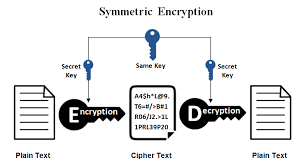
\includegraphics[scale=0.75]{images/sym.png}
	\caption{Szimmetrikus titkosítási algoritmusok működése \cite{ssl2buywiki}.}
	\label{fig:sym_encryption}
\end{figure}

\subsection{AES (Advanced Encryption Standard)}
\noindent Bevált, megbízható titkosítási módszer. 
\vspace{5pt}\\Komplex, több fázisból álló matematikai számításokat hajt végre \cite{nechvatal2001report}.
\vspace{5pt}\\Hátránya, hogy szoftveresen nehezen implementálható lehet. Komplexitása és nagysága miatt teljesítményi ideje is nagy lehet.
\vspace{5pt}\\Úgynevezett 'block cipher', azaz blokk titkosítás. A titkosítandó adatokat blokkokra osztja, egy blokk mérete 128 bit.
\vspace{5pt}\\3 verziója létezik:
\begin{itemize}
	\item AES-128 – 128 bit nagyságú titkosítási kulcsot alklamaz.
	\item AES-192 – 192 bit nagyságú titkosítási kulcsot alkalmaz.
	\item AES-256 – 256 bit nagyságú titkosítási kulcsot alkalmaz.
\end{itemize}
\vspace{5pt}Számítást bájtokon nem pedig biteken végez. 128 bites blokkot az algoritmus 16 bájtként kezel. Ezt a 16 bájtot 4 sorba és oszlopba rendezi a mátrixműveletekhez.
\vspace{5pt}\\Kulcs méretétől függ, hogy hány kört fog az algoritmus elvégezni. 128 bites kulcs – 10 kör, 192 bites kulcs – 12 kör, 256 bites kulcs – 14 kör.
\vspace{5pt}\\Mindegyik kör egy másik 128 bites kulcsot használ, amit az eredeti AES kulcsból számolnak ki.



\subsection{DES (Data Encryption Standard)}
\noindent Block cipher, egy blokk 64 bit nagyságú \cite{standard1999data}.
\vspace{5pt}\\64 bit nagyságú sima szöveg titkosítás után 64bit nagyságú titkosított szöveget eredményez.
\vspace{5pt}\\16 sorozatot véget el matematikai számításokból, mindegyikhez külön titkosítási kulcsot használ.
\vspace{5pt}\\Kulcsok mérete 56 bit (64 bit, de 8-at közülük nem használ).
\vspace{5pt}\\Hátránya lehet, hogy a titkosítás és visszafejtés ugyanazzal az algoritmussal és kulcsokkal történik.
\vspace{5pt}\\Feistel kódon alapszik.



\subsection{Triple DES}
\noindent Működése megegyezik a DES működésével.
\vspace{5pt}\\$3 \times 16$ sorozatot végez, így biztonságosabbnak mondható \cite{enwiki:1078804116}.
% TODO: Mit jelentene az itt, hogy sorozatot végez?
\vspace{5pt}\\Hátránya lehet, hogy a titkosítás és visszafejtés ugyanazzal az algoritmussal és kulcsokkal történik.



\subsection{Blowfish}
\noindent Block cipher, 64 bit méretű blokkok \cite{nie2009study}.
\vspace{5pt}\\ Kulcsok mérete 32 bittől 448 bit-ig terjed, változó méretűek, így lehetőséget nyújt személyes és ipari felhasználásra is. Úgynevezett alkulcsokat is használ (subkey), számszerint 18-at.
\vspace{5pt}\\ Sokkal gyorsabb mint a DES és Triple DES.









\Section{Aszimmetrikus titkosítási algoritmusok}
\noindent Egy privát és egy publikus kulcsot használ \cite{yassein2017comprehensive}.
\vspace{5pt} \\A publikus kulcs lehetővé teszi, hogy bárki titkosítsa az adatokat.
\vspace{5pt} \\A privát kulcs szükséges az adatok  dekódolásához. 
\vspace{5pt} \\Biztonságosabbnak vélhető, mivel a privát kulcsok nem kerülnek megosztásra, de u\-gyan\-ak\-kor nagyobb a számítási költsége is.\newline
\vspace{5pt}\\ Aszimmetrikus algoritmusok általános működési elve a \ref{fig:asym_encryption} ábrán látható.
\begin{figure}[h]
	\centering
	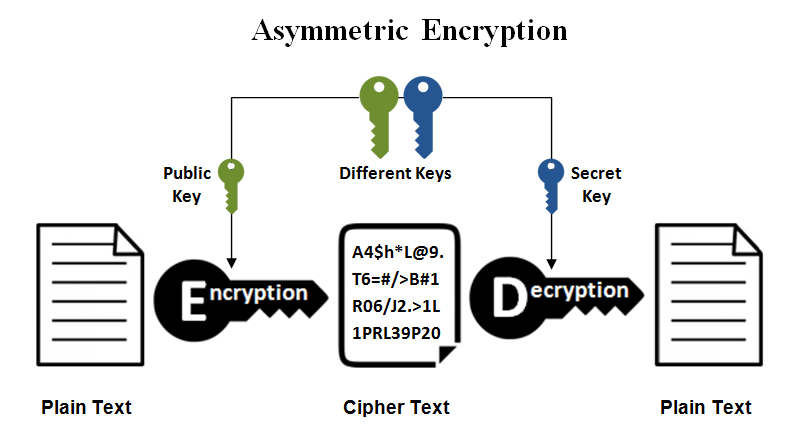
\includegraphics[scale=0.5]{images/asym.png}
	\caption{Aszimmetrikus titkosítási algoritmusok működése \cite{ssl2buywiki}.}
	\label{fig:asym_encryption}
\end{figure}

\subsection{RSA (Rivest–Shamir–Adleman)}
\noindent Azon az elven alapul, hogy a nagy számok szorzása könnyű, de a nagy számok tényezőkre bontása nehéz \cite{gupta2011ecc}. 
\vspace{5pt}\\ A publikus kulcs két számból áll, ami közül az egyik két nagy prímszám szorzata.
\vspace{5pt}\\ A privát kulcs egyik száma ugyanennek a két prímnek a szorzata.


\subsection{DSA (Digital Signature Algorithm)}
\noindent Digitális aláírások titkosítására használt szabvány. Digitális üzenet hitelesítésére is alkalmas \cite{yassein2017comprehensive}.
\vspace{5pt}\\ Moduláris exponenciáláson (modular exponentiation) alapul, a diszkrét logaritmus (discrete logarithm) problémájával együtt.
\vspace{5pt}\\ Privát kulcsot egy üzenet digitális aláírásárának generálására használják. Ellenőrizni az aláíró publikus kulcsával lehetséges.


\subsection{ECC (Elliptic Curve Cryptography)}
\noindent RSA-val vetélkedő aszimmetrikus titkosítási módszer \cite{gupta2011ecc}.
\vspace{5pt}\\ Kulcs generálása matematikai elliptikus görbék segítségével történik.
\vspace{5pt}\\ Alapvető kulcs méret 256 bit, de görbétől függően változhat.

\Section{Hash, hashelés, hash algoritmusok}
A titkosítási módszerek közül kimaradt, az úgynevezett 'hashing', vagy hashelés. Nem sorolható kimondottan sem az adatbázis sem a fájlrendszerek titkosításához. 
\vspace{5pt} \\Érzékeny adatok titkosítására használják, leggyakrabban jelszavakhoz \cite{dang2008recommendation}.
\vspace{5pt} \\Egyediek és ismételhetőek, ami azt jelenti, hogy egy szó ugyanazzal a hash algoritmussal transzformálva ugyanazt a titkosított szöveget fogja eredményezni. 
\vspace{5pt} \\Egy algoritmus mindig ugyanolyan méretű kimenetet állít elő. 
\vspace{5pt} \\Nagyon nehéz két olyan különböző szót találni, amelyek ugyanazon hash algoritmussal transzformálva ugyanazt a titkosított szöveget eredményeznék.
\vspace{5pt} \\Egy hash algoritmussal transzformált szöveget visszaalakítani egyszerű, értelmes szöveggé (plain text) már nem lehet, éppen ezért használják jelszavak titkosítására.
\vspace{5pt} \\Nem visszaalakíthatósága miatt egyezőség vizsgálatát lehet megnézni két ugyanazon hash algoritmussal transzformált, kódolt szöveg között. Ha két hash egyezik, akkor ugyan az volt a bemeneti érték, ha nem egyeznek, akkor különbözőek voltak.
\vspace{5pt} \\Úgynevezett salt és pepper –rel szokás a hasheket ellátni, magasabb biztonság elérése érdekében.
\vspace{5pt} \\ \underline{Salt:} A titkosítandó szövegrészhez extra szöveg csatolása bonyolultság növeléséhez. Regisztrációkor lehet például az email címet és jelszót kombinálni, majd a kombinált szövegen elvégezni a hash algoritmust. Ilyen adatokat 'salted hash'-nek nevezünk.
\vspace{5pt} \\ \underline{Pepper:} Salted hash adathoz, tehát már titkosított adathoz fűz további értékeket. Egy adatbázis esetében ez általában megegyező értéket jelent, azaz minden hashelt adathoz ugyanaz a pepper érték adja hozzá.

A következőkben a két leggyakrabban implemntált hash algoritmust áthatjuk.

\SubSection{MD5 (Message Digest 5)}
Régebben gyakran használt funkció, ami egy 128 bites kimenetet állít elő \cite{gupta2014review}.
\vspace{5pt} \\Kiderült róla, hogy nem ütközésálló (\textit{collision resistant}), emiatt kriptográfusok más hash algoritmusokat ajánlanak. Egy hash függvényre akkor mondjuk, hogy ütközésálló, hogyha nehéz olyan két különböző bemenetet találni, amely ugyanazt a kimenetet eredményezi.


\SubSection{SHA (Secure Hashing Algorithm) Family}

Hat különböző hash függvényből áll: SHA-0, SHA-1, SHA-224, SHA-256, SHA-384, SHA-512 \cite{dang2008recommendation}.
\vspace{5pt} \\Változó méretű bemenetet alakítanak fix méretű kiementté.
\vspace{5pt} \\Az első négy 512 bites blokkokat használ 32 bites szavakra osztva, az utolsó kettő pedig 1024 bites blokkokat 64 bites szavakra bontva.
\vspace{5pt} \\Kimenet mérete SHA-0 és 1 esetén 160 bit, SHA-224 esetén 224 bit, SHA-256 esetén 256 bit, SHA-384 esetén 384 bit, SHA-512 esetén 512 bit nagyságú.
\vspace{5pt} \\Mindegyik algoritmus hasonlóképpen működik.
\vspace{5pt} \\Eredmény mindig 160 bit hosszú. Eredeti üzenet hosszának kevesebbnek kell lennie, mint $2^{64}$-en bit.
\vspace{5pt} \\A SHA-2 családot, aminek a 256, 384, 512 is a tagja, szélés körben implementálták biztonsági alkalmazásokban és protokollokban, mint a TLS, SSL, PGP, stb.
\vspace{5pt} \\A SHA-256-ot a Debian szoftvercsomag hitelesítésére használják és DKIM üzenetaláírási standard. Linux és Unix gyártók 256 és 512 bites SHA-2 használatára tértek át a biztonságos jelszótároláshoz.
\vspace{5pt} \\Számos kriptovaluta, köztük a Bitcoin is használja a SHA-256-ot.


\vspace{25pt}
\Section{Mérések, összehasonlítások}

A mérések végzéséhez az alkalmazásomból elmentett adatokat fogom tesztadatként használni. Az adatokat struktúrált xml dokumentum formátumban kerülnek tárolásra az összehasonlítások elvégzése érdekében. Három különböző méretű fájlt vizsgálunk. Reális méretű fájlok használatára törekedtem (~500KB, ~2MB ~4MB). Már a 4 MB nagyság (nem titkosított) elérését a program rendeltetésszerű használata esetén is elég valószínűtlen tartom, mivel nagyon sok random adatot kellett bemásoljak ahhoz, hogy elérjem ezt a fájlméretet. 
\vspace{5pt}\\Feltehető a mérési eredmények arányos növekedése nagyobb fájlméret esetén.

\subsection{Tesztprogram}
\vspace{5pt}\noindent A mérések összeállítása előtti próbálgatásaimból megtudtam, hogy a titkosítási és visszafejtési idő (a program kód alapján, a \texttt{System.currentTimeMillis()} parancs használatával) nem mindig egyezik meg ugyanazon fájl többszöri titkosítása esetén. Ebből következik, hogy egy adott fájl titkosítását mindegyik algoritmus használatakor többször is el kell végeznem, hogy egy korrekt közelítő értéket kapjak.
\vspace{5pt}\\A tesztprogram elkészítésére elsősorban a \texttt{javax.crypto} és \texttt{java.security} könyvtárakat használtam. A program szempontjából ezen könyvtárak által szolgáltatott fontosabb
% TODO: A programkódra jellemző neveket módszeresen tt-vel kellene szedni!
 \underline{interface-ek}:
\vspace{5pt}\\\textit{Key}: Az összes kulcs legfelső szintű interface-e. Meghatározza az összes kulcs objektum által használt funkciókat.
\vspace{5pt}\\PrivateKey: Célja, hogy csoportosítsa az összes privát kulcs interface-t. Nem tartalmaz metódusokat vagy konstansokat. Speciális privát kulcs interface-ek kiterjesztik ezt az interface-t. 
\vspace{5pt}\\PublicKey: Célja, hogy csoportosítsa az összes nyilvános kulcs interface-t. Nem tartalmaz metódusokat vagy konstansokat. Speciális nyilvános kulcs interface-ek kiterjesztik ezt az interface-t. \newline

\noindent \underline{Osztályok}:
\vspace{5pt}\\-SecretKeySpec: Használható titkos kulcs létrehozására byte tömbből anélkül, hogy SecretKeyFactory-t kellene hozzá használni. ’Nyers’ titkosítási kulcsok számára különösen hasznos, amelyek ábrázolhatók byte tömbként és nincs hozzájuk kulcsparaméter társítva.
\vspace{5pt}\\KeyPair: Egy kulcspár (egy nyilvános és egy privát kulcs) egyszerű tárolója.
\vspace{5pt}\\KeyGenerator: Egy titkos (szimmetrikus) kulcsgenerátor funkcionalitását biztosítja.
\vspace{5pt}\\KeyPairGenerator: Nyilvános és privát kulcspárok létrehozására szolgál.
\vspace{5pt}\\Cipher: Kriptográfiai titkosítási funkciókat biztosít titkosításhoz és visszafejtéshez. A Java Cryptographic Extension (JCE) keretrendszer magját képzi. \newline

\vspace{10pt} \noindent A tesztprogram felépítése hasonló szimmetrikus és aszimmetrikus titkosítás esetén is, néhány eltéréssel.
\\A tesztprogram teljesen reprodukálható a felsorolt osztályok és interface-ek használatával.
\vspace{5pt}\\ Lényegi különbség a két alkalmazás között (szimmetrikus és aszimmetrikus) a kulcsok méretében, létrehozásában / generálásában rejlik. A kódrészletekbe nem megengedett az ékezetes betűk használata, ezért ékezet nélkül kerültek bele magyar szavak.
\vspace{5pt}\\ - Fájl elérési útvonal, jelen esetben a vizsgált xml fájlok útvonala, amik a tesztek készítésekor az asztalomon voltak.
\begin{java}
String filePath = "C:\\Users\\AMD\\Desktop\2MB.xml";
File inputFile = new File(filePath);
\end{java}
\vspace{5pt}- Az objektum és metódus, ami a titkosítást és dekódolást végzi. Az implementálás RSA esetén így nézett ki:
\begin{java}
//Titkositas
Cipher cipher = Cipher.getInstance("RSA");
cipher.init(Cipher.ENCRYPT_MODE, publicKey);
byte[] encryptedFileBytes = cipher.doFinal(inputBytes);

//Visszafejtes
cipher.init(Cipher.DECRYPT_MODE, privateKey);
byte[] decryptedFileBytes = cipher.doFinal(inputBytes);
\end{java}
Szimmetrikus algoritmus használata esetén a publicKey és privateKey helyére a létrehozott szimmetrikus kulcsot kell elhelyezni.
\vspace{15pt}\\ - Kódolt byte-ok fájlba írása, majd a dekódolt byte-ok másik fájlba írása kerül bemutatásra. Azért dekódoltam, hogy meggyőződjek róla, hogy semmi hiba nem történt titkosítás és visszafejtés alatt.
\begin{java}
//Titkositott byte-ok irasa
FileOutputStream outputStream = 
			new FileOutputStream(encryptedFile);
outputStream.write(encryptedFileBytes);
	
//Dekodolt byte-ok irasa
outputStream = new FileOutputStream(decryptedFile);
outputStream.write(decryptedFileBytes);
	
//Ezek lezarasa a megfelelo helyen
outputStream.close();
inputStream.close();
\end{java}
\vspace{5pt}- Az eltelt idő mérésére az említett System.currentTimeMillis() funkció:
\begin{java}
//Kezdo ertek
long start = System.currentTimeMillis();
//Vegso ertek
long end = System.currentTimeMillis();	
//Korrekt idotartam megkapasa
long finalTime = end2-start2;	
\end{java}
A kezdő és végérték inicializálását a megfelelő helyekre kell elhelyezni. Titkosítás és visszafejtés esetén is a kezdőértéket a Cipher objektum létrehozása elé raktam, a kulcs létrehozását nem számítottam bele az időbe. A végértéket a titkosított/dekódolt byte-ok fájlba történő írása után.
\vspace{15pt} \\Ahol a legnagyobb a kód különbsége, a kulcsok létrehozása. Először is meg kell jegyezzem, hogy két módon lehet megfelelő kulcsokat létrehozni:
\vspace{5pt}\\ A megfelelő generátor objektummal (szimmetrikus - KeyGenerator, aszimmetrikus - KeyPairGenerator).
\vspace{5pt}\\ Létrehozni egy String-et, majd abból egy Key objektumot a SecretKeySpec osztály segítségével.
\vspace{5pt}\\Az aszimmetrikus algoritmusok méréséhez az első verziót alkalmaztam, a szimmetrikus algoritmusokhoz pedig a másodikat.
\vspace{5pt}\\ \noindent -Szimmetrikus algoritmus méréseknél a kulcs létrehozása a következő módon nézett ki DES használata esetén:
\begin{java}
String key = "T@stK#Y1";
//Titkos kulcs letrehozasa
Key secretKey = new SecretKeySpec(key.getBytes(), "DES");
\end{java}
Az alkalmazás többi részében a secretKey objektumot kellett használni.
\vspace{7pt}\\- Aszimmetrikus algoritmusok mérésekor a következő volt a kód:
\begin{java}
KeyPairGenerator generator = 
			KeyPairGenerator.getInstance("RSA");
generator.initialize(2048);
KeyPair pair = generator.generateKeyPair();
	
PrivateKey privateKey = pair.getPrivate();
PublicKey publicKey = pair.getPublic();
\end{java}
Titkosításhoz a publicKey-t kell használni, visszafejtéshez pedig a privateKey-t.


\subsection{Eredmények, következtetések}
A számítógépem paraméterei:
\\ Processzor - AMD Ryzen 5 3600X 6-Core 3.79GHz
\\ RAM - 16 GB
\\ OS - Windows 10 Home 64 - bit
\vspace{10pt}\\ Az előzőleg ismertetett szimmetrikus titkosítási algoritmusok tulajdonságainak összehasonlítását tartalmazza a \ref{tab:sym_algorithm_comparison}-es táblázat.
\begin{table}[H]
	\centering
	\caption{Ismertetett szimmetrikus titkosítási algoritmusok összehasonlítása}
	\label{tab:sym_algorithm_comparison}
	\medskip
	
	\begin{tabular}{|p{2.4cm}|p{2.7cm}|p{2.7cm}|p{2.7cm}|p{2.7cm}|}
		\hline
		 & \textbf{AES} & \textbf{DES} & \textbf{Triple DES}  & \textbf{Blowfish} \\
		\hline
		Lehetséges kulcs méret(ek) & 128/192/256 bit & 64 bit (56-ot használ) & Összesen 168 bit & Mérete 32 bittől 448 bitig terjedhet \\
		\hline
		Mekkora egy block mérete? & 128 bit & 64 bit & 64 bit & 64 bit \\
		\hline
		Hány kört végez az algoritmus? & Kulcs méretétől függ  & 16 kör & $3 \times 16$ kör & 16 kör \\
		 & 128 bit - 10 kör & & & \\
		 & 192 bit - 12 kör & & & \\
		 & 256 bit - 14 kör & & & \\
		\hline
		Külön kulcsot használ-e minden körben? & Igen, mindegyik kör más kulcsot használ. & Igen, különböző 48 bites kulcsokat. & Három különböző DES kulcsot. & Igen, 32 bit nagyságúakat. \\
		\hline
		Sikerült-e már feltörni? & Nem. & Igen, úgynevezett brute force támadással. & Vegyes válaszokat találtam, de mivel már nem igazán használják csak régebbi szoftverek, és a DES is fel lett törve, ezért valószínűleg \textbf{igen}. & Nem. \\
		\hline
	\end{tabular}
\end{table}
\noindent Úgy gondolom, hogy az algoritmusok biztonságával kapcsolatosan megfelelő méréseket nem tudok végezni, ezért nem szerepelnek a dokumentumban. A táblázat ’Sikerült-e már feltörni’ sorában lévő információk is az interneten talált adatok, ezekből lehet valamilyen szinten az algoritmus biztonságára vonatkoztatni.\newline

\noindent Az előző alfejezetben bemutatott tesztprogramot használva megvizsgáltam 500kb, 1mb, 2mb, 3mb és 4mb nagyságú fájl titkosításának sebességét a szimmetrikus algoritmusokat használva. A \ref{tab:enc_500kb}-es, \ref{tab:dec_500kb}-as, és \ref{tab:enc_1mb}-től \ref{tab:dec_4mb}-ig tartó táblázatok a mérések eredményeit tartalmazzák.
\noindent \\ Az AES algoritmusok 128 bit nagyságú kulcsot használtak. \\A táblázatokban szereplő értékek milliszekundumban (ms) értendők.
\vspace{5pt}
\begin{table}[H]
	\centering
	\caption{500KB-hoz tartozó titkosítási mérések}
	\label{tab:enc_500kb}
	\medskip
	\begin{tabular}{|p{2.4cm}|p{2cm}|p{2cm}|p{2cm}|p{2cm}|}
		\hline
		\textbf{Titkosítás} \newline \textbf{500KB} & \textbf{AES} & \textbf{DES} & \textbf{Triple DES} & \textbf{Blowfish}\\
		\hline
		\textbf{1.mérés} & 49 & 51 & 73 & 48\\
		\hline
		\textbf{2.mérés} & 44 & 50 & 69 & 44\\
		\hline
		\textbf{3.mérés} & 46 & 50 & 70 & 49\\
		\hline
		\textbf{4.mérés} & 43 & 50 & 74 & 49\\
		\hline
		\textbf{5.mérés} & 48 & 56 & 71 & 46\\
		\hline
		\textbf{6.mérés} & 46 & 57 & 74 & 50\\
		\hline
		\textbf{7.mérés} & 44 & 53 & 74 & 52\\
		\hline
		\textbf{8.mérés} & 44 & 57 & 74 & 52\\
		\hline
		\textbf{9.mérés} & 47 & 58 & 70 & 50\\
		\hline
		\textbf{10.mérés} & 61 & 58 & 70 & 46\\
		\hline
		\hline
		\textbf{Átlag} & \textbf{46,2} & \textbf{54} & \textbf{71,9} & \textbf{48,6}\\
		\hline
	\end{tabular}
\end{table}

\begin{table}[H]
	\centering
	\caption{500KB-hoz tartozó visszafejtési mérések}
	\label{tab:dec_500kb}
	\medskip
	\begin{tabular}{|p{2.4cm}|p{2cm}|p{2cm}|p{2cm}|p{2cm}|}
		\hline
		\textbf{Visszafejtés} \newline \textbf{500KB} & \textbf{AES} & \textbf{DES} & \textbf{Triple DES} & \textbf{Blowfish}\\
		\hline
		\textbf{1.mérés} & 7 & 17 & 28 & 14\\
		\hline
		\textbf{2.mérés} & 7 & 21 & 28 & 13\\
		\hline
		\textbf{3.mérés} & 6 & 17 & 29 & 12\\
		\hline
		\textbf{4.mérés} & 7 & 16 & 35 & 13\\
		\hline
		\textbf{5.mérés} & 7 & 17 & 28 & 13\\
		\hline
		\textbf{6.mérés} & 7 & 18 & 35 & 12\\
		\hline
		\textbf{7.mérés} & 8 & 16 & 33 & 14\\
		\hline
		\textbf{8.mérés} & 6 & 20 & 29 & 15\\
		\hline
		\textbf{9.mérés} & 8 & 17 & 29 & 14\\
		\hline
		\textbf{10.mérés} & 8 & 19 & 30 & 14\\
		\hline
		\hline
		\textbf{Átlag} & \textbf{7,2} & \textbf{17,8} & \textbf{30,4} & \textbf{13,4}\\
		\hline
	\end{tabular}
\end{table}


\noindent A fájl mérete titkosítás előtt és után minden esetben megegyezett, kivéve pár bájt különbséget.
\vspace{5pt} \\Az átlagértékeket a \ref{tab:avg_enc}-es és \ref{tab:avg_dec}-ös táblázatokba gyűjtöttem össze jobb átláthatóság érdekében.
\begin{table}[H]
	\centering
	\caption{Titkosítási átlagértékek}
	\label{tab:avg_enc}
	\medskip
	\begin{tabular}{|p{2.4cm}|p{2.7cm}|p{2.7cm}|p{2.7cm}|p{2.7cm}|}
		\hline
		\textbf{Titkosítás}& \textbf{AES} & \textbf{DES} & \textbf{Triple DES}  & \textbf{Blowfish} \\
		\hline
		\textbf{500KB}&46,2 ms&54 ms&71,9 ms&48,6 ms \\
		\hline
		\textbf{1MB}&54,2 ms&67,7 ms&104,4 ms&59,2 ms \\
		\hline
		\textbf{2MB}&56,7 ms&88,6 ms&153,9 ms&69,8 ms \\
		\hline
		\textbf{3MB}&61,1 ms&110,5 ms&217,4 ms&82,7 ms \\
		\hline
		\textbf{4MB}&63,2 ms&132 ms&269,2 ms&93,7 ms \\
		\hline
	\end{tabular}
\end{table}


\begin{table}[H]
	\centering
	\caption{Visszafejtési átlagértékek}
	\label{tab:avg_dec}
	\medskip	
	\begin{tabular}{|p{2.4cm}|p{2.7cm}|p{2.7cm}|p{2.7cm}|p{2.7cm}|}
		\hline
		\textbf{Visszafejtés}& \textbf{AES} & \textbf{DES} & \textbf{Triple DES}  & \textbf{Blowfish} \\
		\hline
		\textbf{500KB}&7,2 ms&17,8 ms&30,4 ms&13,4 ms \\
		\hline
		\textbf{1MB}&12 ms&29,9 ms&59,3 ms&19,2 ms \\
		\hline
		\textbf{2MB}&18 ms&48,5 ms&115,7 ms&33 ms \\
		\hline
		\textbf{3MB}&21,2 ms&67,9 ms&174 ms&42,4 ms \\
		\hline
		\textbf{4MB}&23 ms&85 ms&229,1 ms&50,7 ms \\
		\hline
	\end{tabular}
\end{table}


\noindent Néhány esetben viszonylag nagy eltérés volt az értékek között, például a Triple DES esetében, a 4MB méret 5.mérése (lásd \ref{tab:enc_4mb} táblázat) ~50 milliszekundummal nagyobb mint a többi mérés. Pontosabb átlagértékeket kaphatnánk, ha egy módszerrel X méretű fájlt százszor titkosítanánk, nem pedig csak tízszer, és az így kapott eredményeket átlagolnánk.
\vspace{5pt}\\Ettől függetlenül az így kapott értékekről lehet következtetéseket levonni.
\vspace{5pt}\\Mindkét téren (titkosítás és visszafejtés) az AES használata bizonyult a leggyorsabbnak (lásd \ref{tab:avg_enc} és \ref{tab:avg_dec} táblázat). Ahogy a fájl mérete nőtt, úgy az AES titkosítási ideje nem nőtt olyan látványosan, mint a többi algoritmus esetében. Visszafejtési időre szintén igaz ez az állítás. 
\vspace{5pt}\\Gyorsaságot tekintve legközelebb az AES-hez a Blowfish állt, mind visszafejtés és titkosítás terén is. 
\vspace{5pt}\\A DES és a Triple DES közötti egyre inkább növekvő különbség várható volt, hiszen a Triple DES háromszor végzi el azt, amit a DES csak egyszer. Ennek ellenére titkosítási időben nem érte el a Triple DES az elődje háromszorosát, habár nagyobb fájlméret esetén a növekedésüket nézve valószínűleg el fogja, sőt ezt a tendenciát követve valószínűleg a különbség több, mint a háromszorosára is nőhet. Visszafejtési időben sokkal inkább látszik ez a különbség, 4 MB-os fájl titkosítása átlagosan kétszer addig tart a Triple DES-nek, mint a DES-nek, visszafejtést nézve 4 MB esetén ez az érték majdnem háromszorosára nőtt (lásd \ref{tab:avg_enc} és \ref{tab:avg_dec} táblázat).
\vspace{5pt}\\ Az átlagértékek szemléltetésére grafikonok is készültek, amik a \ref{fig:alg_titkositas_graf} és \ref{fig:alg_visszafejtes_graf}-es ábrán láthatók. A függőleges tengely a titkosítási időket tartalmazza milliszekundumban mérve, a vízszintes tengely pedig a fájlok méretét.
\begin{figure}[H]
	\centering
	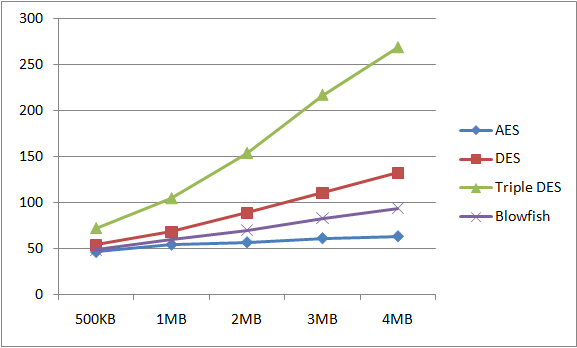
\includegraphics[scale=0.8]{images/alg_graf_1.png}
	\caption{Szimmetrikus titkosítási mérések}
	\label{fig:alg_titkositas_graf}
\end{figure}

\begin{figure}[H]
	\centering
	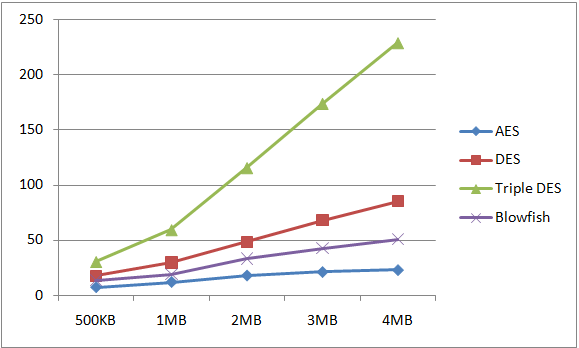
\includegraphics[scale=0.8]{images/alg_graf_2.png}
	\caption{Szimmetrikus visszafejtési mérések}
	\label{fig:alg_visszafejtes_graf}
\end{figure}


\vspace{5pt} \noindent A program szempontjából valószínűtlennek tartom a 4MB-nál nagyobb fájl lehetőségét, de a mérések kedvéért 64MB nagyságú fájl titkosítását is elvégeztem ugyanilyen módon. 
A kapott értékek a \ref{tab:enc_64mb}-as és \ref{tab:dec_64mb}-es táblázatokban láthatók, amik szintén milliszekundumban értendők.
\begin{table}[H]
	\centering
	\caption{64MB-hoz tartozó titkosítási mérések}
	\label{tab:enc_64mb}
	\medskip
	\begin{tabular}{|p{2.4cm}|p{2cm}|p{2cm}|p{2cm}|p{2cm}|}
		\hline
		\textbf{Titkosítás} \newline \textbf{64MB} & \textbf{AES} & \textbf{DES} & \textbf{Triple DES} & \textbf{Blowfish}\\
		\hline
		\textbf{1.mérés} & 392 & 1678 & 3505 & 956\\
		\hline
		\textbf{2.mérés} & 369 & 1314 & 3524 & 950\\
		\hline
		\textbf{3.mérés} & 359 & 1703 & 3522 & 968\\
		\hline
		\textbf{4.mérés} & 411 & 1688 & 3512 & 993\\
		\hline
		\textbf{5.mérés} & 364 & 1676 & 3515 & 979\\
		\hline
		\textbf{6.mérés} & 377 & 1682 & 3514 & 974\\
		\hline
		\textbf{7.mérés} & 354 & 1311 & 3514 & 974\\
		\hline
		\textbf{8.mérés} & 374 & 1328 & 4351 & 974\\
		\hline
		\textbf{9.mérés} & 377 & 1693 & 3518 & 1089\\
		\hline
		\textbf{10.mérés} & 366 & 1694 & 3501 & 997\\
		\hline
		\hline
		\textbf{Átlag} & \textbf{374,3} & \textbf{1576,6} & \textbf{3597,6} & \textbf{985,4}\\
		\hline
	\end{tabular}
\end{table}

\begin{table}[H]
	\centering
	\caption{64MB-hoz tartozó visszafejtési mérések}
	\label{tab:dec_64mb}
	\medskip
	\begin{tabular}{|p{2.4cm}|p{2cm}|p{2cm}|p{2cm}|p{2cm}|}
		\hline
		\textbf{Visszafejtés} \newline \textbf{64MB} & \textbf{AES} & \textbf{DES} & \textbf{Triple DES} & \textbf{Blowfish}\\
		\hline
		\textbf{1.mérés} & 298 & 1301 & 3451 & 735\\
		\hline
		\textbf{2.mérés} & 314 & 1272 & 3464 & 775\\
		\hline
		\textbf{3.mérés} & 300 & 1323 & 3516 & 755\\
		\hline
		\textbf{4.mérés} & 297 & 1297 & 3452 & 762\\
		\hline
		\textbf{5.mérés} & 289 & 1305 & 3447 & 747\\
		\hline
		\textbf{6.mérés} & 289 & 1309 & 3438 & 755\\
		\hline
		\textbf{7.mérés} & 285 & 1560 & 3441 & 767\\
		\hline
		\textbf{8.mérés} & 401 & 1297 & 4269 & 763\\
		\hline
		\textbf{9.mérés} & 308 & 1299 & 3435 & 764\\
		\hline
		\textbf{10.mérés} & 291 & 1298 & 3453 & 750\\
		\hline
		\hline
		\textbf{Átlag} & \textbf{307,2} & \textbf{1326,1} & \textbf{3536,6} & \textbf{757,3}\\
		\hline
	\end{tabular}
\end{table}


\noindent A 4MB-os táblázatok értékeivel összehasonlítva ezeket az értékeket a következőt kapjuk:
\vspace{5pt}\\Az AES titkosítási ideje 5,92-szeresére nőtt, amíg a visszafejtési ideje 13,35-szörösére.
\vspace{5pt}\\A DES titkosítási ideje 11,94-szeresére nőtt, amíg a visszafejtési ideje 15,6-szorosára.
\vspace{5pt}\\A TripleDES titkosítási ideje 13,36 -szorosára nőtt, amíg a visszafejtési ideje 15,44-szeresére.
\vspace{5pt}\\A Blowfish titkosítási ideje 10,51-szeresére nőtt, amíg a visszafejtési ideje 14,94- szeresére.
\vspace{5pt}\\Ezek az adatok azért lehetnek érdekesek, mivel ha a 4MB és 64MB-os fájlméretet nézzük, akkor igaz, hogy 64 / 4 = 12, így ezt a logikát követve 12-szeres időnövekedést várhatunk titkosítás és visszafejtés esetén is. Ennek ellenére nem ezt kapjuk, hol többet, hol kevesebbet, tehát az egyenes arányosság logikája nem alkalmazható az algoritmusok idejének becslésére.
\vspace{5pt}\\Ezt az állítást igazolhatjuk az 500KB-1MB-2MB-4MB-os táblázatokat nézve is, mivel ezekben a táblázatokban sem duplázódtak meg pontosan az idők, annak ellenére, hogy a fájl mérete dupla akkora lett.



\newpage \noindent  A 64 MB-os esethez külön diagramot készítettem, különben a skálázás miatt a kisebb méretű fájlok értékei alig látszottak volna (lásd \ref{fig:alg_64mb_graf} ábra).
\begin{figure}[h]
	\centering
	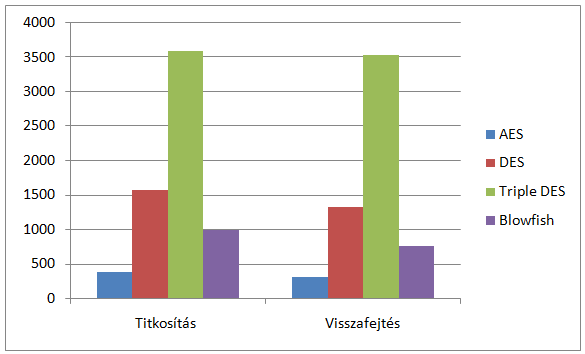
\includegraphics[scale=0.8]{images/alg_graf_3.png}
	\caption{64MB-os fájl titkosítás, visszafejtés. Függőleges tengely - idő (ms)}
	\label{fig:alg_64mb_graf}
\end{figure}

\vspace{25pt} \noindent \underline{Aszimmetrikus titkosítási algoritmusok:}
\vspace{15pt} \\ \textbf{RSA}
\vspace{5pt} \\ Szerettem volna a szimmetrikus algoritmusokkal összehasonlítani, de nem lenne korrekt, mivel az adatmennyiség felsőhatára, amit a javax.crypto könyvtár használatával titkosítani tudtam 245 byte volt. Ha nagyobb mérettel próbálkoztam hibaüzenetet kaptam „Data must not be longer than 245 bytes”.
\vspace{5pt} \\Ezután az interneten jobban utána olvastam a problémának és megtudtam, hogy az RSA algoritmus maximum akkora mennyiségű adatot képes titkosítani, mint az RSA kulcs mérete (mínusz az ún. header data, azaz fejlécadat). 
\vspace{5pt} \\Kettő hatványait használtam kulcsméret megadására, először 2048 bit nagy\-sá\-gú kulcs\-csal kezdtem.
\\Az eredmények milliszekundumban értendők és a \ref{tab:enc_rsa}-as és \ref{tab:dec_rsa}-es táblázatban találhatók.

\begin{table}[H]
	\centering
	\caption{RSA titkosítási mérések különböző méretű fájlokkal}
	\label{tab:enc_rsa}
	\medskip
	\begin{tabular}{|p{2.4cm}|p{2cm}|p{2cm}|p{2cm}|p{2cm}|}
		\hline
		\textbf{Titkosítás} \newline \textbf{RSA} & \textbf{64 byte} & \textbf{128 byte} & \textbf{245 byte}\\
		\hline
		\textbf{1.mérés} & 28 & 24 & 28\\
		\hline
		\textbf{2.mérés} & 28 & 24 & 30\\
		\hline
		\textbf{3.mérés} & 25 & 26 & 30\\
		\hline
		\textbf{4.mérés} & 23 & 26 & 28\\
		\hline
		\textbf{5.mérés} & 24 & 25 & 28\\
		\hline
		\textbf{6.mérés} & 26 & 21 & 25\\
		\hline
		\textbf{7.mérés} & 27 & 23 & 22\\
		\hline
		\textbf{8.mérés} & 30 & 28 & 22\\
		\hline
		\textbf{9.mérés} & 29 & 26 & 21\\
		\hline
		\textbf{10.mérés} & 25 & 28 & 25\\
		\hline
		\hline
		\textbf{Átlag} & \textbf{26,5} & \textbf{25,1} & \textbf{25,9}\\
		\hline
	\end{tabular}
\end{table}

\begin{table}[H]
	\centering
	\caption{RSA visszafejtési mérések különböző méretű fájlokkal}
	\label{tab:dec_rsa}
	\medskip
	\begin{tabular}{|p{2.4cm}|p{2cm}|p{2cm}|p{2cm}|p{2cm}|}
		\hline
		\textbf{Visszafejtés} \newline \textbf{RSA} & \textbf{64 byte} & \textbf{128 byte} & \textbf{245 byte}\\
		\hline
		\textbf{1.mérés} & 7 & 6 & 7\\
		\hline
		\textbf{2.mérés} & 6 & 5 & 4\\
		\hline
		\textbf{3.mérés} & 6 & 7 & 5\\
		\hline
		\textbf{4.mérés} & 4 & 7 & 7\\
		\hline
		\textbf{5.mérés} & 6 & 7 & 6\\
		\hline
		\textbf{6.mérés} & 7 & 4 & 4\\
		\hline
		\textbf{7.mérés} & 5 & 7 & 9\\
		\hline
		\textbf{8.mérés} & 7 & 7 & 5\\
		\hline
		\textbf{9.mérés} & 8 & 5 & 7\\
		\hline
		\textbf{10.mérés} & 7 & 8 & 6\\
		\hline
		\hline
		\textbf{Átlag} & \textbf{6,3} & \textbf{6,3} & \textbf{6}\\
		\hline
	\end{tabular}
\end{table}

\noindent Ezután megpróbáltam nagyobb fájlokat titkosítani, így növelnem kellett a kulcs nagyságát is.
\vspace{5pt} \\ A kulcs nagysága: 8192 bit. Titkosítandó fájl nagysága: 1013 byte (a fejlécadat nagysága miatt ez lett a limit, de a kettőt összeadva egyébként $2^{10}$-en, azaz 1024 byte). Titkosított fájl mérete: 1024 byte. Az eredmények  \aref{tab:rsa_1024byte} táblázatban találhatók. A 4 különböző fájl átlagértékei grafikonos formában \aref{fig:rsa_graf}-as ábrán láthatók.

\begin{table}[H]
	\centering
	\caption{RSA titkosítás és visszafejtés 1024 byte nagyságú fájl esetén}
	\label{tab:rsa_1024byte}
	\medskip
	\begin{tabular}{|p{2.4cm}|p{2.4cm}|p{2.4cm}|}
		\hline
		\textbf{1024 byte} & \textbf{Titkosítás} & \textbf{Visszafejtés}\\
		\hline
		\textbf{1.mérés} & 28 & 117\\
		\hline
		\textbf{2.mérés} & 21 & 123\\
		\hline
		\textbf{3.mérés} & 22 & 121\\
		\hline
		\textbf{4.mérés} & 31 & 121\\
		\hline
		\textbf{5.mérés} & 29 & 125\\
		\hline
		\textbf{6.mérés} & 23 & 119\\
		\hline
		\textbf{7.mérés} & 24 & 122\\
		\hline
		\textbf{8.mérés} & 27 & 121\\
		\hline
		\textbf{9.mérés} & 28 & 119\\
		\hline
		\textbf{10.mérés} & 23 & 124\\
		\hline
		\hline
		\textbf{Átlag} & \textbf{25,6} & \textbf{121,1}\\
		\hline
	\end{tabular}
\end{table}


\noindent Annak ellenére, hogy ezek az értékek nem  tűnnek nagynak, a számítógépemnek elég sokáig tartott minden mérés elvégzése, volt néhol 10 másodperc is, mire az eredményt megkaptam. Mivel már az 1 kb-os fájl titkosítása is eddig tartott, nagyobb méretű fájllal nem próbálkoztam.
\begin{figure}[h]
	\centering
	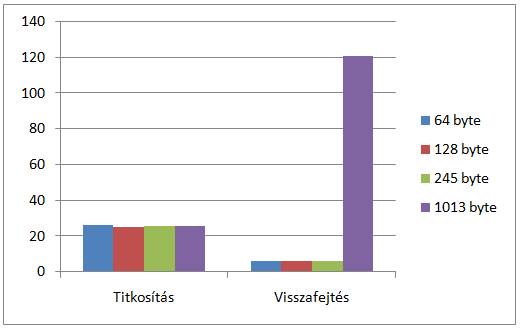
\includegraphics[scale=0.8]{images/alg_graf_4.png}
	\caption{RSA titkosítás, visszafejtés. Függőleges tengely - idő (ms)}
	\label{fig:rsa_graf}
\end{figure}
\\ \noindent DSA mérését és összehasonlítását nem tartom korrektnek, mivel nem nagy méretű adat titkosítására, hanem digitális aláírásokra lett kifejlesztve.
\vspace{5pt}\\ECC mérést szintén nem készítettem, mivel nem tudtam. Utánanéztem az interneten és ECC titkosítást elméletileg a \texttt{javax.crypto} könyvtár segítségével nem lehet végrehajtani. Más függvény könyvtárat azért nem használtam, mert úgy gondolom fennáll a lehetősége, hogy eltérnek az algoritmusok implementálásai, így olyan könyvtár használata lenne optimális, amely az összes vizsgált algoritmust tartalmazza.



\vspace{15pt}\noindent Röviden összefoglalva, a tesztekkel és mérésekkel olyan eredményeket kaptam, amikre számítottam, annak ellenére, hogy a sebességük az előző alfejezetek leírásaiban nem lett számszerűsítve. 
\\Az AES-nél nem értek egyet a talált állítással, miszerint "Hátránya, hogy szoftveresen nehezen implementálható lehet, illetve komplexitása és nagysága miatt teljesítményi ideje is nagy lehet".
\\A szoftveres implementálás függvény könyvtár használata miatt volt egyszerű, a matematikai részét nem nekem kellett megoldanom.
\\Nagy teljesítményi ideje pedig relatív, hiszen a többi vizsgált szimmetrikus algoritmushoz képest az AES-é volt a legkisebb.
	\Chapter{Tervezés}

Ez a fejezet a program tervezésével kapcsolatos információkat, specifikációkat tartalmazza. Egy látványterv leírása a felhasználói felületről és a szükséges funkciókról.

\Section{A grafikus felhasználói felület tervei}

Az alkalmazás két menüpontből álljon, jegyzetek és kereső menü. A két menü működése egyedi objektumok használatával történjen.

% TODO: Minden subsection-t javtani kellene SubSection-re!

\subsection{Szükséges adattípusok}
Szükséges egy Note és egy Page objektum konstruktor létrehozása.

A Note objektumnak legyenek a következő változói:
\begin{itemize}
	\item String noteName - A jegyzet neve.
	\item ArrayList<Page> pageList - Egy Page típusú ArrayList a jegyzet oldalainak tárolására. Egyszerűen lehet majd törölni és hozzáadni új Page objektumokat.
	\item int Id - Egy ID az egyszerű azonosítás érdekében.
	\item static int counter - Egy számláló, ami majd az ID-t növeli, maga a számláló értékét pedig a konstruktorban kell növelni.
	\item Minden adathoz a megfelelő getter-setter metódusok.
\end{itemize}

\vspace{10pt} \noindent A Page objektumnak legyenek a következő változói:
\begin{itemize}
	\item String pageName - Az oldal neve.
	\item String pageText - Az oldal tartalma, a szövegdobozba írt adatok.
	\item int noteId - A lapot tartalmazó jegyzet ID-je ahhoz, hogy egyszerűen meghatározható legyen a kapcsolat egy Note és egy Page objektum között.
	\item int Id - Egy ID az egyszerű azonosítás érdekében.
	\item static int counter - Egy számláló, ami majd az ID-t növeli, maga a számláló értékét pedig a konstruktorban kell növelni.
	\item Minden adathoz a megfelelő getter-setter metódusok.
\end{itemize}

\subsection{Közös elemek}

A következő elemek olyanok, amelyeknek mindkét menüpontban látszaniuk kell és használhatóak kell legyenek. \Aref{fig:main_foundation}. ábrán pirossal bekeretezett és számozott részek ezeket az elemeket jelzik, leírásuk számozva a továbbiakban következnek.

\begin{figure}[h]
	\centering
	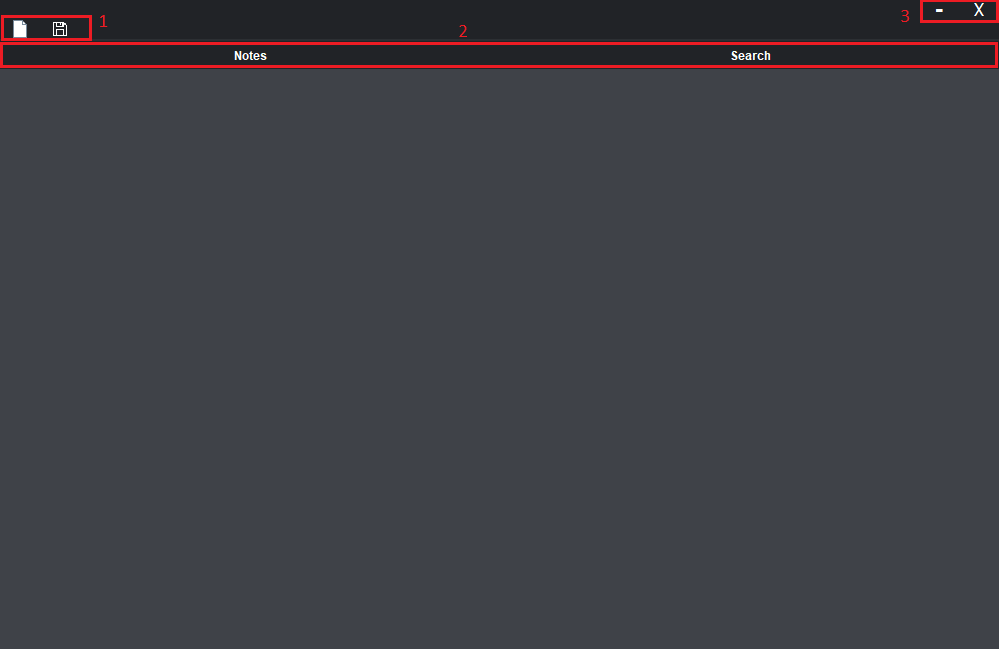
\includegraphics[scale=0.5]{images/menu_1.png}
	\caption{Program 'körvonala', alapja, a felület amire a többi menü épül.}
	\label{fig:main_foundation}
\end{figure}

\noindent \textbf{1.} Gombok helye. Fájl megnyitása és mentése gombra gondoltam. Ha további gombok hozzáadása szükséges lenne,  azok is ide kerülnének, feltéve ha mindegyik menüpontban használhatóak.
\vspace{5pt} \\Fájl megnyitása gomb (4.1 ábrán az 1.ikon): lokális adatbázis használata esetén lehet fontos. Szükségessége attól függ, hogy lokális vagy felhőalapú adatbázis kerül felhasználásra.
\vspace{5pt} \\Fájl mentése gomb (4.1 ábrán a 2. ikon): elmenti az adatok változásait, amiket a későbbiekben az adatbázisba kell töltsön.
\vspace{5pt} \\ \textbf{2.} Két menüpont váltására alkalmas gombok helye, ezekre kattintva válthatunk a menük között.
\vspace{5pt} \\ \textbf{3.} Bezár és tálcáz gombok, funkcióik egyértelműeknek tartom.
\vspace{10pt} \\Az alkalmazás ablak bárhová legyen elhelyezhető a képernyőn (tehát lehessen húzgálni), amíg a felső sötétebb színű sávon tartjuk lenyomva  a bal egérgombot, viszont átméretezni ne lehessen.
\vspace{5pt} \\Belépéskor ez a kép fogadja a felhasználót, egyik menüpontban se legyen benne. 

\subsection{Jegyzetek menü}

\Aref{fig:menu_notes}. ábrán látható a jegyzetek menü elképzelt felépítése A pirossal számozott elemek leírása található a következőkben, amely elmondja, hogy milyen funkciókat kell majd, hogy az egyes elemek betöltsenek.

\begin{figure}[h]
	\centering
	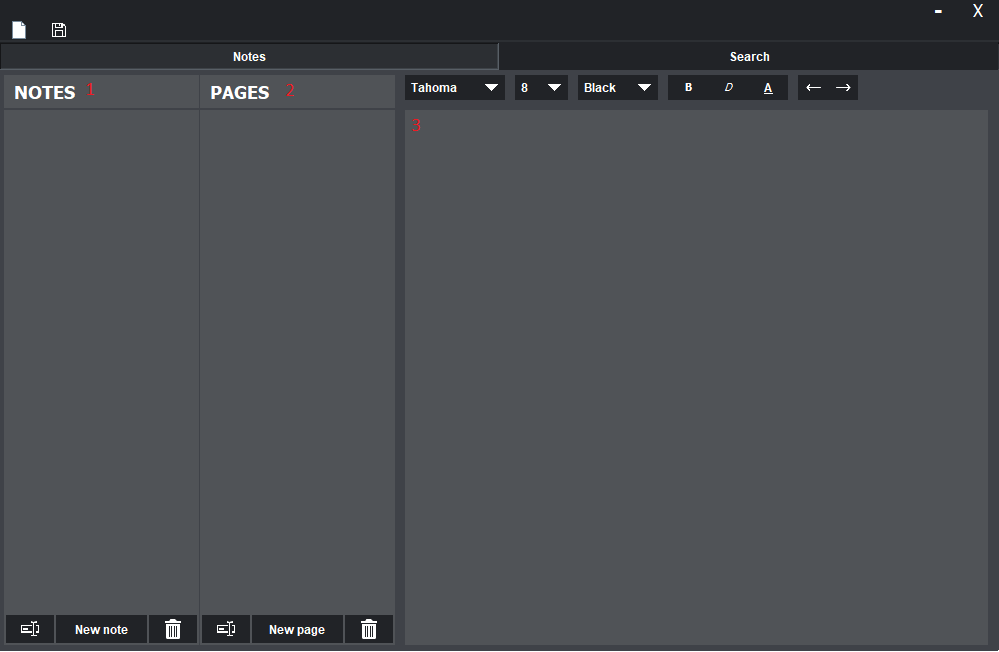
\includegraphics[scale=0.5]{images/menu_2.png}
	\caption{Jegyzetek menü}
	\label{fig:menu_notes}
\end{figure}

\vspace{5pt} \noindent \textbf{1.} Jegyzetek (Note objektumok) listája, ahol a jegyzetek neve jelenik meg egymás alatt. 
\\Ha betelne a jegyzetek listája, akkor a görgő segítségével lehet köztük navigálni.
\\Átnevezni, létrehozni és törölni jegyzeteket a lista alján található gombokkal lehessen. A gombok csak a kijelölt jegyzetet szerkesszék!
\vspace{5pt} \\ \textbf{2.} Oldalak (Page objektumok) listája. Ha nincs jegyzet kiválasztva, akkor a lista alapvetően üres legyen. Az éppen kijelölt (rákattintott) jegyzet oldalainak nevei legyenek itt felsorolva. 
\\Egy jegyzethez több oldal is létrehozható, de egy adott oldal csak egy meghatározott jegyzethez tartozhat (feltéve ha nem másoltuk be egy másik jegyzetbe ugyan azt a szöveget és adtunk a lapunknak hasonló címet). 
\\Ha betelne az oldalak listája, akkor a görgő segítségével lehessen köztük navigálni. 
\\Átnevezni, létrehozni és törölni oldalakat a lista alján található gombokkal lehetséges. A gombok csak a kijelölt oldalakat szerkesszék!
\\Ha nincs kijelölve jegyzet, akkor a lapok listája is legyen üres.
\vspace{5pt} \\ \textbf{3.} Szövegszerkesztő, az éppen kijelölt oldal tartalma legyen itt látható és szerkeszthető. 
\\Ha nincs oldal kijelölve, akkor ne legyen használható a szerkesztő és ne jelenjen meg benne szöveg. 
\vspace{5pt} \\Legyenek elérhetők szöveg szerkesztésére alkalmas gombok, amelyek funckiói a következők: 
\begin{itemize}
	\item Betűstílus, betűméret és szín megadására alkalmas legördülő választási menü.
	\item Szöveg dőltté, vastaggá és aláhúzottá alakító gombok. Ki-bekapcsolóként működjenek.
	\item Undo gomb, ami az előző szerkesztést vonja vissza.
	\item Redo gomb, ami az előzőleg visszavont szerkesztést csinálja újra.
\end{itemize}
Az első és második pontban leírt funkcióknak csak a kijelölt szövegen legyen hatása.
\\A gombok legyenek gyorsbillentyűkkel is használhatók.


\subsection{Kereső menü}

A \ref{fig:menu_search}. ábrán látható a kereső menü elképzelt felépítése A pirossal számozott elemek leírása található a későbbiekben, hogy részletezze, hogy milyen funkciókat kell majd, hogy az egyes elemek betöltsenek.

\begin{figure}[h]
	\centering
	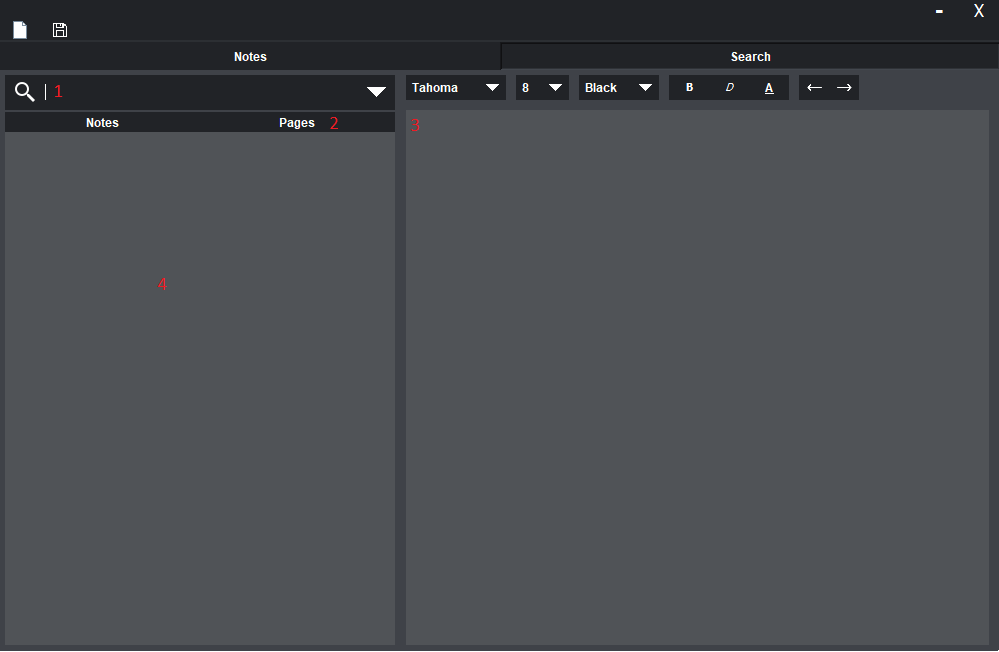
\includegraphics[scale=0.5]{images/menu_3.png}
	\caption{Kereső menü}
	\label{fig:menu_search}
\end{figure}

\vspace{5pt} \noindent \textbf{1.} Kereső sáv. Ne legyen case-sensitive, tehát ne tegyen kis- és nagybetű között különbséget.
\\Jegyzet- és oldalnevek, és az oldalak tartalma között is keressen egyező adatokat.
\\Jelenjen meg egy legördülő menü ahogy írjuk a szöveget, ami a találatok nevét tartalmazza. Tehát ha egyezést talál a beírt szöveg és 
\begin{itemize}
	\item egy jegyzet neve között, akkor a jegyzet neve jelenjen meg.
	\item egy lap neve között, akkor a lap neve jelenjen meg.
	\item egy lap tartalma között, akkor a tartalmazó lap neve jelenjen meg.
\end{itemize}
Beírt szövegre a nagyító gombra való kattintással tudjunk keresni, vagy a legördülő menüben megjelenő találatokra kattintva. 
\vspace{5pt} \\ \textbf{2.} Talált jegyzetek és lapok között a két adott gombbal lehessen váltani. Jelenjen meg a kiválasztott találatok listája.
\\Gombra való kattintással lehessen kiválasztani hogy melyik lista látszódjon.
\vspace{5pt} \\ \textbf{3.} A jegyzetek menünél bemutatott szövegszerkesztő, melynek működése legyen megegyező.
A kijelölt lap szövege jelenjen meg itt, legyen szerkeszthető.
\vspace{5pt} \\ \textbf{4.} A 2. pontban jellemzett gombok esetén két lehetőség legyen: vagy a jegyzetek listája látszódjon, vagy a lapok listája. 
\\A listák az érvényes találatokat tartalmazzák.
\\Lehessen a listák elemei között (úgy mint a jegyzetek menüben) kattintással választani. Ilyenkor további két lehetőség legyen:
\begin{itemize}
	\item Ha egy jegyzet listaelemet választunk, akkor a program tegyen át a jegyzetek menüpontba, és legyen a kiválasztott jegyzet kijelölve. Ha a jegyzetet görgetéssel lehet elérni, akkor a görgő is legyen a megfelelő pozícióba úgy, hogy látszódjon a listán a kiválasztott elem. Lapja ne legyen kijelölve, szövegdoboz legyen üres.
	\item Ha egy lap listaelemet választunk, akkor a szövegdobozban jelenjen meg a  tartalma. Legyen itt is szerkeszthető a tartalom.
\end{itemize}

\Section{Adatbázis}
Az adatok adatbázisba legyenek eltárolva, vagy felhőalapú adatbázisba, vagy lokális adatbázisba. 
\\Ha lokális adatbázisra esik a választás, az adatok szinkronizálása több eszköz között legyen megoldva.
\\Adatbázishoz való csatlakozás a programkódban legyen megfelelően implementálva.


\Section{Titkosítás}
A titkosítási algoritmus tesztek alapján a legjobbnak vélt algoritmussal kerüljenek az adatok kódolásra.
\\A titkosítás vagy alkalmazás szinten, saját implementációval legyen megoldva vagy a tárolástól függően az ismertetett adatbázis titkosítási módszerek egyikének alkalmazásával.
\\Mivel az alkalmazás minden esetben az adathalmaz egészével dolgozik, ezért elegendő lehet, ha egy XML vagy JSON fájl kerül titkosításra, amely az összes adatot tartalmazza, nem pedig minden adat egyesével.
\\A titkosítási kulcsok legyenek biztonságosan tárolva, több eszköz között biztonságosan megosztva.
\\Az alkalmazás bezárása előtt kerüljenek át az adatok az adatbázisba. Alkalmazás megnyitása után kerüljenek beolvasásra majd megjelenítésre.

	\Chapter{Implementáció}

A fejezet a program készítése során felmerülő problémák leírásával foglalkozik. Bemutatja hogyan sikerült az alkalmazás egyes részeit implementálnom. Nem tartalmaz a program használatával kapcsolatos információkat. 
\\A fejezet felépítése a program csomag-szintű felépítésével egyezik.
% \\Nem \LaTeX\-Java stílusú kódrészleteket tartalmaz, hanem beszúrt képeket a kész kódról.

\Section{Data}

Az előző fejezetben leírt szükséges adattípusokat egy Content nevű osztályba gyűjtöttem össze. A csomag felépítése \aref{fig:package_data}. ábrán látható.
\vspace{5pt}\\Két tároló objektumot tartalmaz, amelyek DefaultListModel típusúak, ezen belül Note és Page típusú adatokat tartalmaznak. DefaultListModel objektumot egy lista elemeinek létrehozására és megjelenítésére használjuk Java-ban. Mivel az adatok csak listákban kerülnek megjelenítésre, ezért ez az objektum tökéletes volt az adatok tárolására.
\vspace{5pt}\\Az alkalmazás azon részei, amelyek az adatokkal dolgoznak a Content osztályon keresztül érik el őket.
\begin{figure}[h]
	\centering
	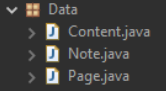
\includegraphics[scale=0.7]{images/package_data.png}
	\caption{Data csomag és osztályai}
	\label{fig:package_data}
\end{figure}

\Section{Database}
Egy osztályt tartalmaz, a DatabaseFunctions-t, amiben az adatbázissal kapcsolatos funkciókat gyűjtöttem össze, mint az adatbázishoz való csatlakozás, fájlok fel- és letöltése. A csomag felépítése a \ref{fig:package_database}. ábrán látható.
\vspace{5pt}\\Az adatok Firebase nevű felhőalapú adatbázisban kerülnek tárolásra, így az alkalmazás megfelelő működéséhez szükséges van internetkapcsolatra.
\\Az alkalmazást át kellett alakítanom Maven project-re, hogy a Firebase adatbázis driver-éhez hozzá tudjak férni, majd az API segítségével kapcsolatba tudjak lépni az adatbázissal.
\\Lehetsőségünk van Firebase-en belül Blob (Binary large object/Nagy bináris objektum) fájlok tárolására. Az alkalmazás adatai titkosított XML fájl formájában kerülnek az adatbázisba. A Firebase ezen felül data-at-rest titkosítást is alkalmaz.
\begin{figure}[h]
	\centering
	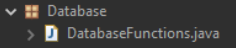
\includegraphics[scale=0.7]{images/package_database.png}
	\caption{Database csomag és osztálya}
	\label{fig:package_database}
\end{figure}

% TODO: Az ilyen képek helyett az osztályokról inkább kisebb UML diagramok kellenének!

\Section{Encryption}
Titkosítással kapcsolatos osztályokat tartalmaz. A csomag felépítése a \ref{fig:package_encryption}. ábrán látható.
\vspace{5pt}\\Az AppKeyStore osztálynak két funkciója van. 
\\Egyik egy random generált 256 bit-es AES titkosítási kulcs létrehozására szolgál, amit egy KeyStore objektumban tárol, ezt .jks kiterjesztésű 256 karakter hosszú jelszóval védett fájlként tárolja. A fájl a progarm működése alatt feltöltődik az adatbázisba.
\\A jelszó karakterek random sorozatából áll, de minden .jks fájl ugyanazzal a jelszóval van védve. Vitatható, hogy ez a megoldás biztonságos-e, úgy gondolom, hogy igen, a jelszó hosszából és karaktereiből ítélve, ugyanis nem csak számokat és betűket tartalmaz, hanem szimbólumokat is.
\\Adatbázisba töltését szükségszerűnek tartom, hogy különböző eszközökön is el tudjuk érni ugyanazt a tartalmat.
\\Másik metódusa segítségével letölti az adatbázisból a .jks fájlt, amit ideiglenesen eltárol az eszközön, majd ebből az ideiglenes fájlból éri el a korábban létrehozott titkosítási kulcsot.
\vspace{5pt}\\Az EncryptionFunctions osztály a titkosítást és visszafejtést végző funkciókat tartalmazza. Ezek a műveletek a .jks fájlba elmentett random generált kulcsot alkalmazzák az XML fájl titkosításához és visszafejtéséhez.
\\A funkciók AES algoritmust használnak, működésük megegyezik az algoritmusok összehasonlításához használt tesztalkalmazás működésével, a javax.crypto csomag osztályait alkalmaztam.

\begin{figure}[h]
	\centering
	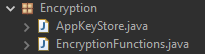
\includegraphics[scale=0.7]{images/package_encryption.png}
	\caption{Encryption csomag és osztályai}
	\label{fig:package_encryption}
\end{figure}

\Section{XML}
A csomag XML-lel foglalkozó osztályokat tartalmaz, felépítése a \ref{fig:package_xml}. ábrán látható. Ilyen az XMLReader, ami olvassa és 'parse'-olja az adott XML fájlt. Az XMLWriter XML dokumentum írását és formázását végzi.
\vspace{5pt}\\A program a szükséges fájlokat egy config.xml-nek nevezett dokumentumból éri el, aminek írását és olvasását a ConfigManager osztály végzi. Ennek az osztálynak a részletes működését a következő fejezet tartalmazza.


\begin{figure}[h]
	\centering
	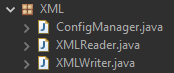
\includegraphics[scale=0.7]{images/package_xml.png}
	\caption{XML csomag és osztályai}
	\label{fig:package_xml}
\end{figure}

\Section{GUI}
Ez a csomag a felhasználói felület főbb osztályait tartalmazza (lásd \ref{fig:package_gui}. ábra).
\vspace{5pt}\\Legnehezebb dolgom a TextEditorButtons nevű osztállyal volt, ami a 4.1.3-mas alfejezetben leírt szövegszerkesztő megfelelő működését biztosítja. A felhasználói felület készítése során ennek az osztálynak létrehozása volt a legidőigényesebb feladat.
\\Alapértelmezett beállítás a 12-es nagyság, fehér szín és Dialog betűstílus. A szövegszerkesztőbe beírt adatok és a szövegszerkesztő gombjai között nincs valós-idejű kapcsolat.
\\Ezt egy példával tudom legjobban elmagyarázni: ha a szöveg egy részének (a gombok ugye csak a kijelölt részeket szerkesztik) stílusát megváltoztatjuk, tegyük fel 18-as betűméret, piros szín és Times New Roman betűstílusra, a gombokon feltüntetett szöveg megváltozik. Ha a kurzorral egy nem szerkesztett szövegrészre kattintunk, akkor a gombok állapota nem áll vissza az alapértelmezett beállításokra, hanem az utoljára beállított opción marad (tehát nem lesz Dialog-12-fehér, hanem Times New Roman-18-piros marad).


\begin{figure}[h]
	\centering
	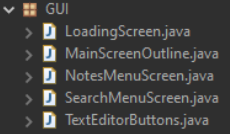
\includegraphics[scale=0.7]{images/package_gui.png}
	\caption{GUI csomag és osztályai}
	\label{fig:package_gui}
\end{figure}


\Section{GUIRelated}
A csomag olyan osztályokat tartalmaz, amelyek a grafikus felhasználói felület személyre szabásában segítettek. A csomag felépítése a \ref{fig:package_guirelated}. ábrán látható.
\begin{figure}[h]
	\centering
	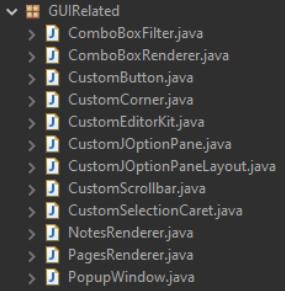
\includegraphics[scale=0.6]{images/package_guirelated.png}
	\caption{GUIRelated csomag és osztályai}
	\label{fig:package_guirelated}
\end{figure}
\\A felhasználói felületet Java Swing használatával készítettem. Ahhoz, hogy megértsük milyen nehézségekkel szembesültem, egy rövid leírásban be kell mutassam a függvénykönyvtárat:
\vspace{10pt}\\A Swing egy GUI widget toolkit. Widget-ek alatt olyan grafikus elemeket értünk, mint gombok, szövegdobozok, listák, legördülő menük, görgők, stb...
\\A Swing egy régi technológia, viszont rengeteg alkalmazás használja. A Java GUI készítésre létrehoztak egy modernebb függvénykönyvtárat, ami a Swing-re épül, a JavaFX-et.
\\Kevésbé használt, mint a Swing, valószínűleg azért, mivel az alkalmazások nagy része korábban, Swing-ben készült, és nincs szükség JavaFX-szé való konvertálásukra. Új Java GUI-k készítésére valószínűnek tartom, hogy inkább JavaFX-et használnak.
\vspace{10pt}\\Azért választottam a Swing-et a JavaFX helyett, mert már dolgoztam a könyvtárral, míg a JavaFX-et egyáltalán nem ismertem, így azt gondoltam, hogy egyszerűbb dolgom lesz.
\\Hamar rá kellett jönnöm, hogy nem lesz olyan egyszerű dolgom, mint amire számítottam, de ettől függetlenül maradtam a Swing használata mellett. Ahhoz, hogy a widget-eknek egy modern megjelenést tudjunk adni, rengeteg szülőosztály-beli metódust kell megvizsgálnunk és felülírnunk. Sok esetben nem érhető el olyan funkció, amit logikusnak tartanánk, hogy létezik és közvetlenül szerkeszthető. Pár példa, hogy mire is gondolok:
\vspace{5pt}\\A JButton widget egy gomb, amire lehet szöveget írni. Ha megnyomjuk a gombot, megváltozik a háttérszíne, amíg el nem engedjük az egérgombot. Ezt a színt közvetlenül egy metódussal nem lehet megváltoztatni. A felülírt kódról egy részlet a \ref{fig:package_guirelated_jbutton}. ábrán látható
\begin{figure}[h]
	\centering
	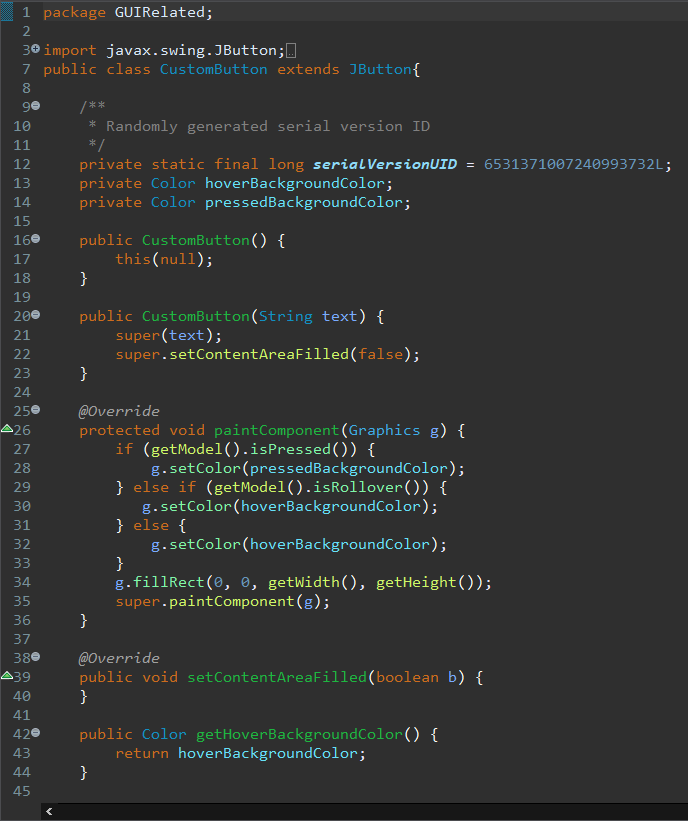
\includegraphics[scale=0.3]{images/package_guirelated_jbutton_details.png}
	\caption{JButton megjelenését felülírő osztály}
	\label{fig:package_guirelated_jbutton}
\end{figure}
\\A JList listaelemek háttérszínét, legyen-e az elemeknek kerete vagy sem, elemek szövegének színét sem lehet közvetlen metódussal megváltoztatni. A felülírt kódról egy részlet a \ref{fig:package_guirelated_jlistrenderer}. ábrán látható
\begin{figure}[h]
	\centering
	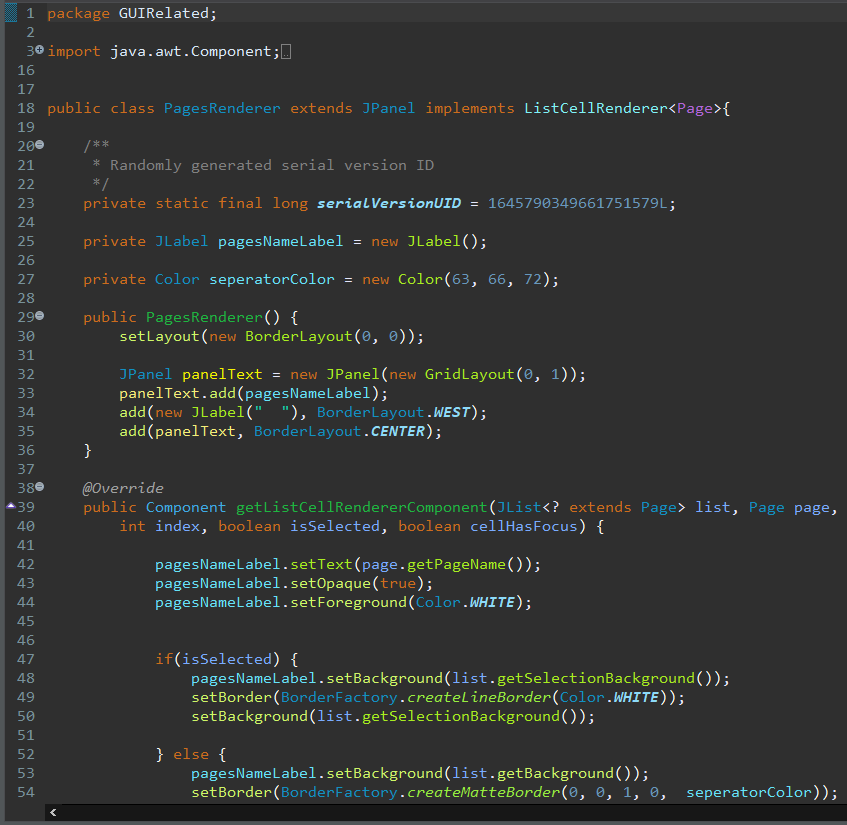
\includegraphics[scale=0.3]{images/package_guirelated_jlistrenderer_details.png}
	\caption{JList listaelemeit renderelő osztály}
	\label{fig:package_guirelated_jlistrenderer}
\end{figure}
\vspace{5pt} \\ \noindent A csomag összes osztálya ilyen jellegű problémákat old meg, szükségesek az elképzelt, modern felhasználói felület létrehozásához.


\Section{Main}
A csomag a fő futtatható osztályt tartalmazza. Internetkapcsolat ellenőrző függvényt és az alkalmazás adatait betöltő algoritmusokat tartalmazza. A csomag felépítése a \ref{fig:package_main}. ábrán látható.

\begin{figure}[h]
	\centering
	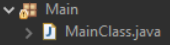
\includegraphics[scale=0.6]{images/package_main.png}
	\caption{Main csomag és osztálya}
	\label{fig:package_main}
\end{figure}


\Section{További fejlesztési lehetőségek}
Egyik opció sem kulcsfontosságú az alkalmazás működésének szempontjából, azért nem kerültek bele a program végső verziójába. Hasznos funkciók, de némelyik inkább csak a kényelmet szolgálja.
\\Az ötletek nagy részének későbbi megvalósítása ettől függetlenül tervbe van.

\subsection{Automatikus elindulás}
A program automatikusan induljon el az eszköz indításakor.

\subsection{Naptár és emlékeztető}
Az első megvalósítandó ötlet egy naptár elhelyezése az alkalmazás kettő meglévő menüje mellé.
\\Ez a képernyő jelenne meg alkalmazás indulásakor, főmenü szerepet töltene be.
\vspace{5pt}\\A felületen lenne egy naptár, amit lehetne időben előre-hátra lapozni, akárcsak egy rendes naptárat.
\vspace{5pt}\\Emlékeztető írására alkalmas funkciókat is kéne tartalmazzon, ez lenne a menüpont lényege. A felhasználó írhatna egy emlékeztetőt egy jövőbeli eseményre (múltbeli eseményre hibát dobna) és be lehetne állítani, hogy mikor emlékeztessen (aznap, egy nappal előtte, két nappal előtte, stb..).
\vspace{5pt}\\Emlékeztető alatt egy felugró ablakra gondolok, ami attól függetlenül, hogy milyen ablakok vannak még megnyitva (legyen az böngésző, vagy másik alkalmazás), azok felett lenne (on top). 
\\Felépítése hasonló lenne a jegyzet/lap törlése modális ablakéhoz.
Tartalmazna egy 'OK' gombot, ami bezárja ezt az ablakot, és egy 'Remind me later' gombot, ami ideiglenesen bezárja az ablakot, majd X perc múlva ismét megjeleníti. A gombok felett jelenne meg az emlékeztető szövege.


\subsection{Beállítások}
Egy felugró ablak, tele opciókkal.
\\Kimondottan a felhasználói felület megváltoztatására alkalmas beállításokra gondolok (pl.: színek variálása), de akár működés	módosítására alkalmas beállításokat is tartalmazhatna ez az ablak.
\\Két titkosítási opciót is el lehetne itt helyezni. Ezalatt arra gondolok, hogy alkalmazás szintű titkosítási megoldást alkalmazzon az applikáció vagy elegendőnek tartja a felhasználó az adatbázis at-rest titkosítását, amit a szolgáltató végez.


	\Chapter{Működés, tesztelés}

A fejezet az elkészített alkalmazás rendeltetésszerű működését mutatja be.

\Section{Config fájl}
Az alkalmazáshoz szükséges fájlok elérési útvonalát a config.xml fájlban kell megadni.
Egy fájl elérési útvonalát az alábbi módon kell megadni: \\C:\textbackslash Users\textbackslash AMD\textbackslash Desktop\textbackslash firebase\_service\_key\_example.json.
\vspace{5pt}\\Ha az alkalmazást először futattjuk az eszközön, vagy egy új mappában tettük a futtatható .jar fájlt, amiben nem található config.xml, akkor automatikusan létrejön az adott mappában egy fájl, példa adatokkal. Ezeket meg kell változtatnunk, hogy használni tudjuk az alkalmazást.
\vspace{15pt}\\A \ref{fig:config_file}. ábra egy automatikusan létrehozott config.xml fájl felépítését mutatja. A pirossal számozott sorok tartalmát kell szerkesszük, a további alfejezetekben ezt fejtem ki.
\begin{figure}[h]
	\centering
	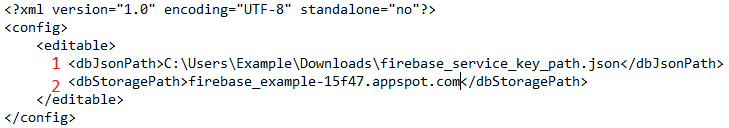
\includegraphics[scale=0.5]{images/config_1.png}
	\caption{Config.xml tartalma első futtatás után}
	\label{fig:config_file}
\end{figure}

\subsection{Firebase}
A \ref{fig:config_file}. ábrán piros 1 és 2-essel jelölt sorok megfelelő kitöltéséhez létre kell hoznunk egy Firebase adatbázist. 
\vspace{5pt}\\Egy böngészőben a \href{https://console.firebase.google.com/u/0/}{console.firebase.google.com} url beírása, majd egy google fiókba való belépés után ez a \ref{fig:firebase_reg}. ábrán látható kép fogad minket.

\begin{figure}[H]
	\centering
	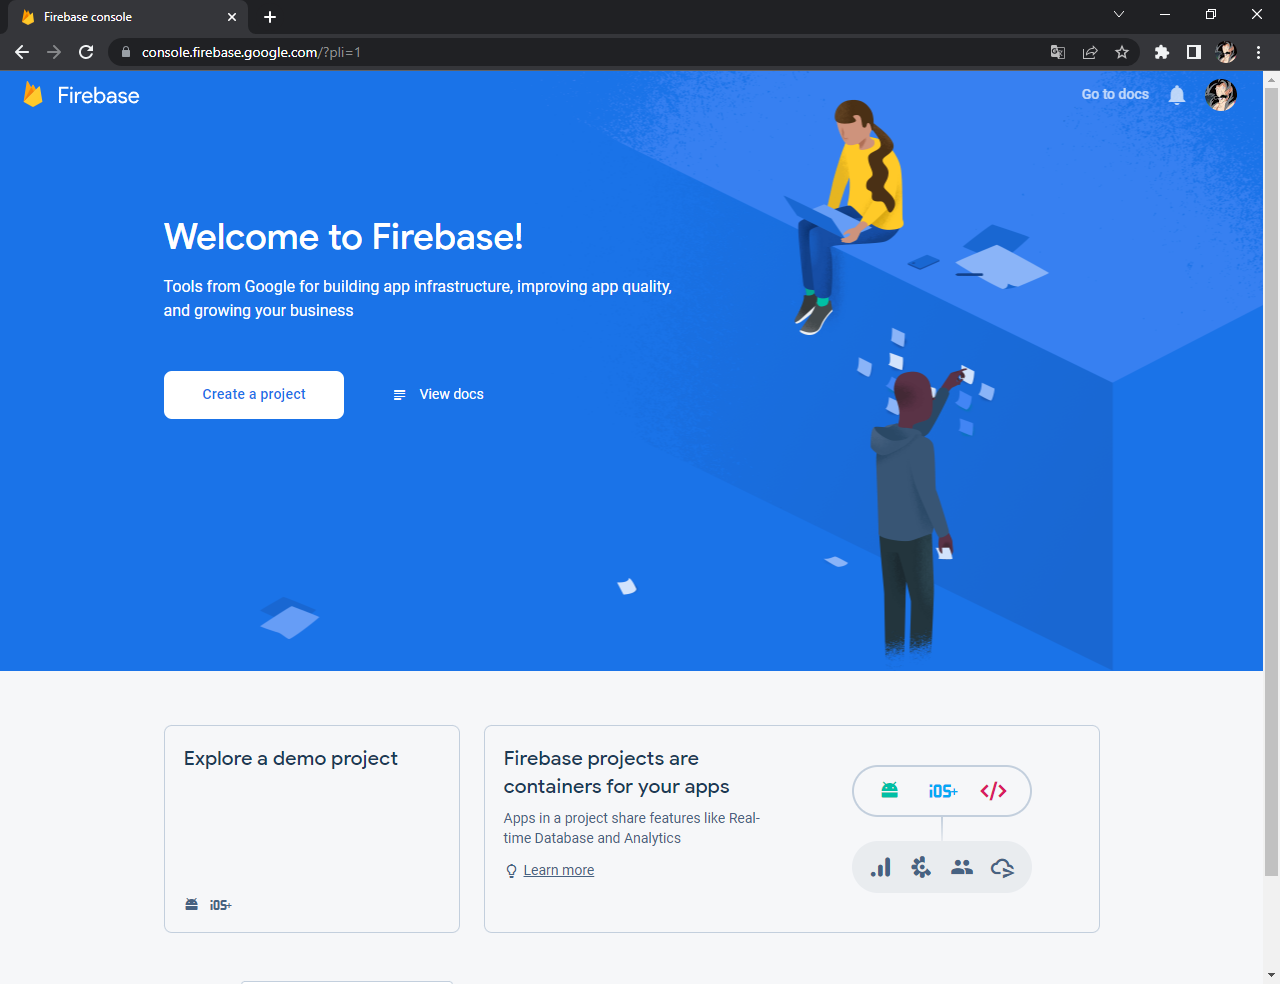
\includegraphics[scale=0.2]{images/config_2.png}
	\caption{Firebase regisztráció}
	\label{fig:firebase_reg}
\end{figure}
\noindent Kattintsunk a 'Create a project' gombra, majd végezzük el a szükséges lépéseket.
\\Ha megtettük, a \ref{fig:firebase_storage_reg}. ábra képét láthatjuk. Kattintsunk a 'Storage' gombra a 'Build' menün belül, a kép bal szélén található sávban.

\begin{figure}[H]
	\centering
	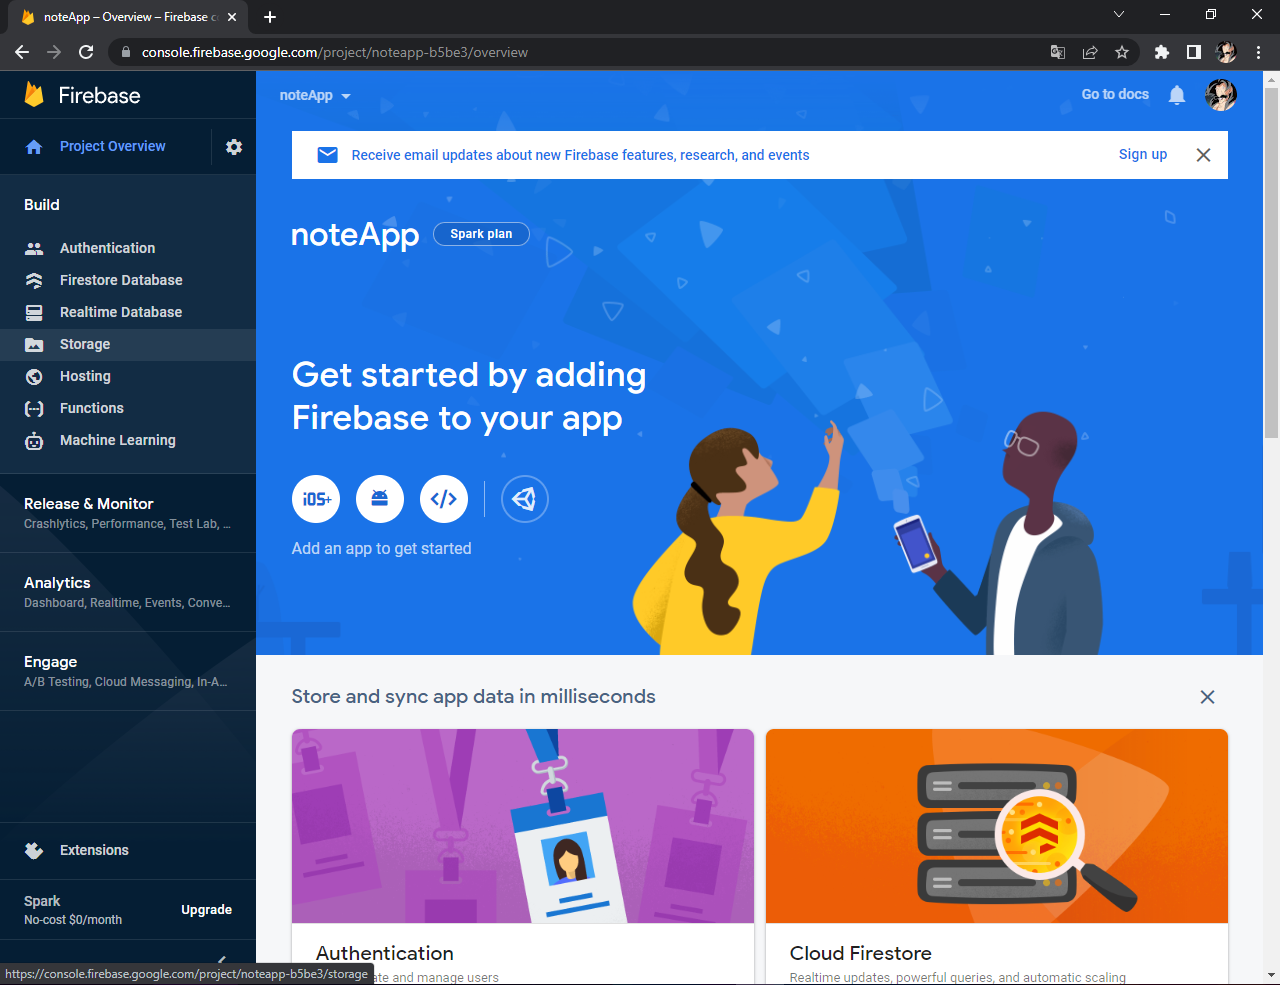
\includegraphics[scale=0.2]{images/config_3.png}
	\caption{Firebase kezdő képernyő}
	\label{fig:firebase_storage_reg}
\end{figure}

\noindent Kattintsunk a 'Get started' gombra, majd válasszuk ki a 'Start in production mode' lehetőséget, majd 'Next'. A legördülő menüben válasszuk a megfelelő Storage location-t, ami valószínűleg eur3 (europe-west) lesz. Fontos, hogy ezt nem lehet később megváltoztatni, így győződjünk meg választásunkról! Végül a 'Done' gombra nyomjunk.
\vspace{5pt}\\Ha ezt mind megtettük a \ref{fig:firebase_storage_default}. ábrához hasonlót látunk.

\begin{figure}[H]
	\centering
	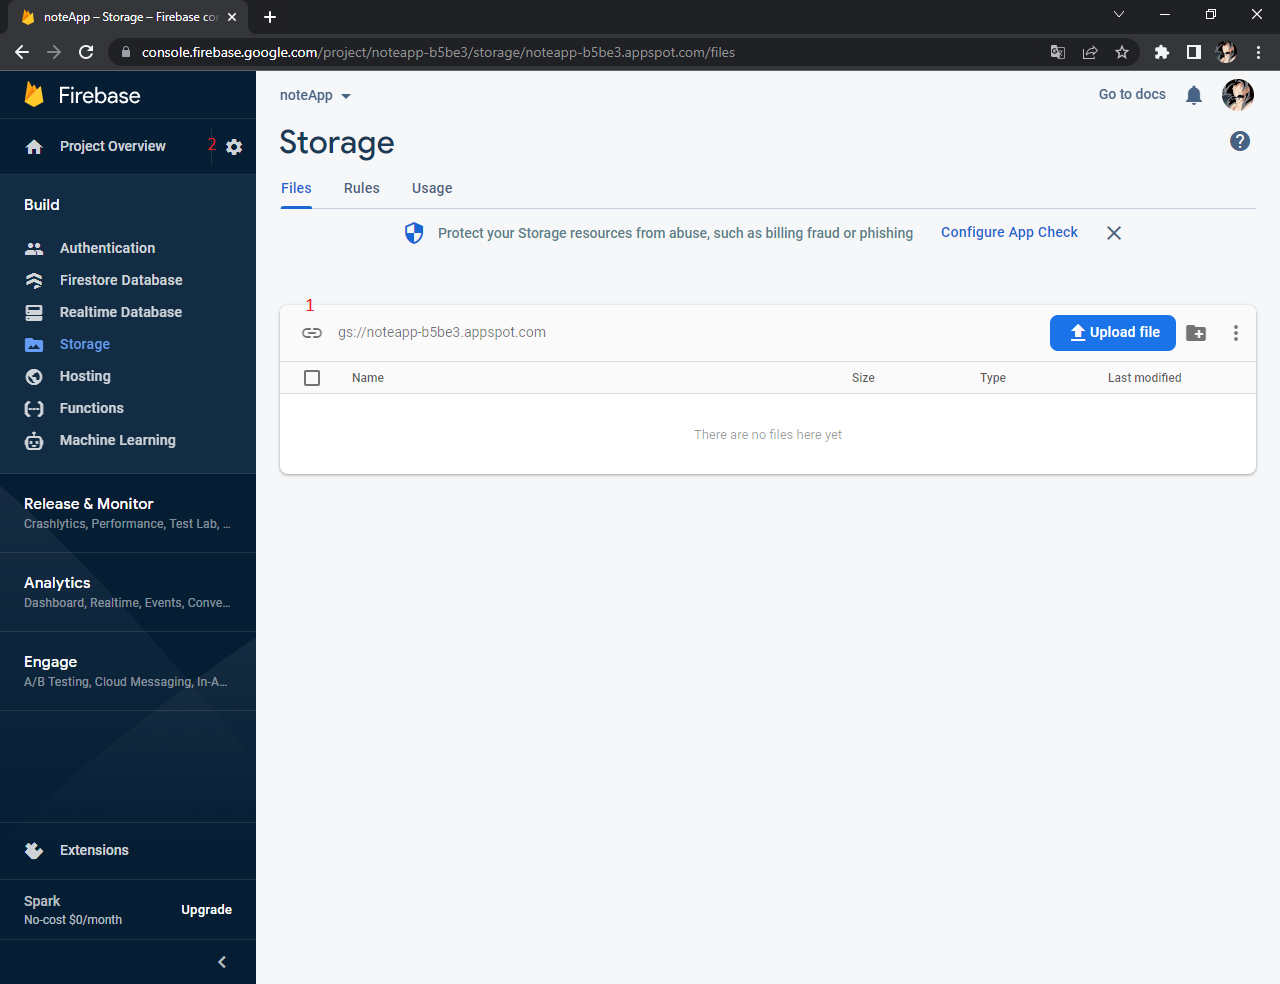
\includegraphics[scale=0.2]{images/config_4.png}
	\caption{Firebase storage alapértelmezett kép}
	\label{fig:firebase_storage_default}
\end{figure}

\noindent A config.xml fájlban a tag-ek (<dbJsonPath>...</dbJsonPath>) közé kell a megfelelő adatokat beírnunk. A \ref{fig:config_file}. ábrán piros 2-essel jelölt <dbStoragePath>...</dbStoragePath> tag-ek közé a \ref{fig:firebase_storage_default}. ábrán 1-essel jelölt linket kell bemásoljuk a 'gs://' nélkül.
\vspace{5pt}\\Ha ez megvan kattintsunk a \ref{fig:firebase_storage_default}. ábrán piros 2-essel jelölt fogaskerékre, majd 'Project settings', az újonnan megjelent felső sávban pedig a service accounts-ra (lásd \ref{fig:firebase_service_key}. ábra 3-mas lehetőség).

\begin{figure}[H]
	\centering
	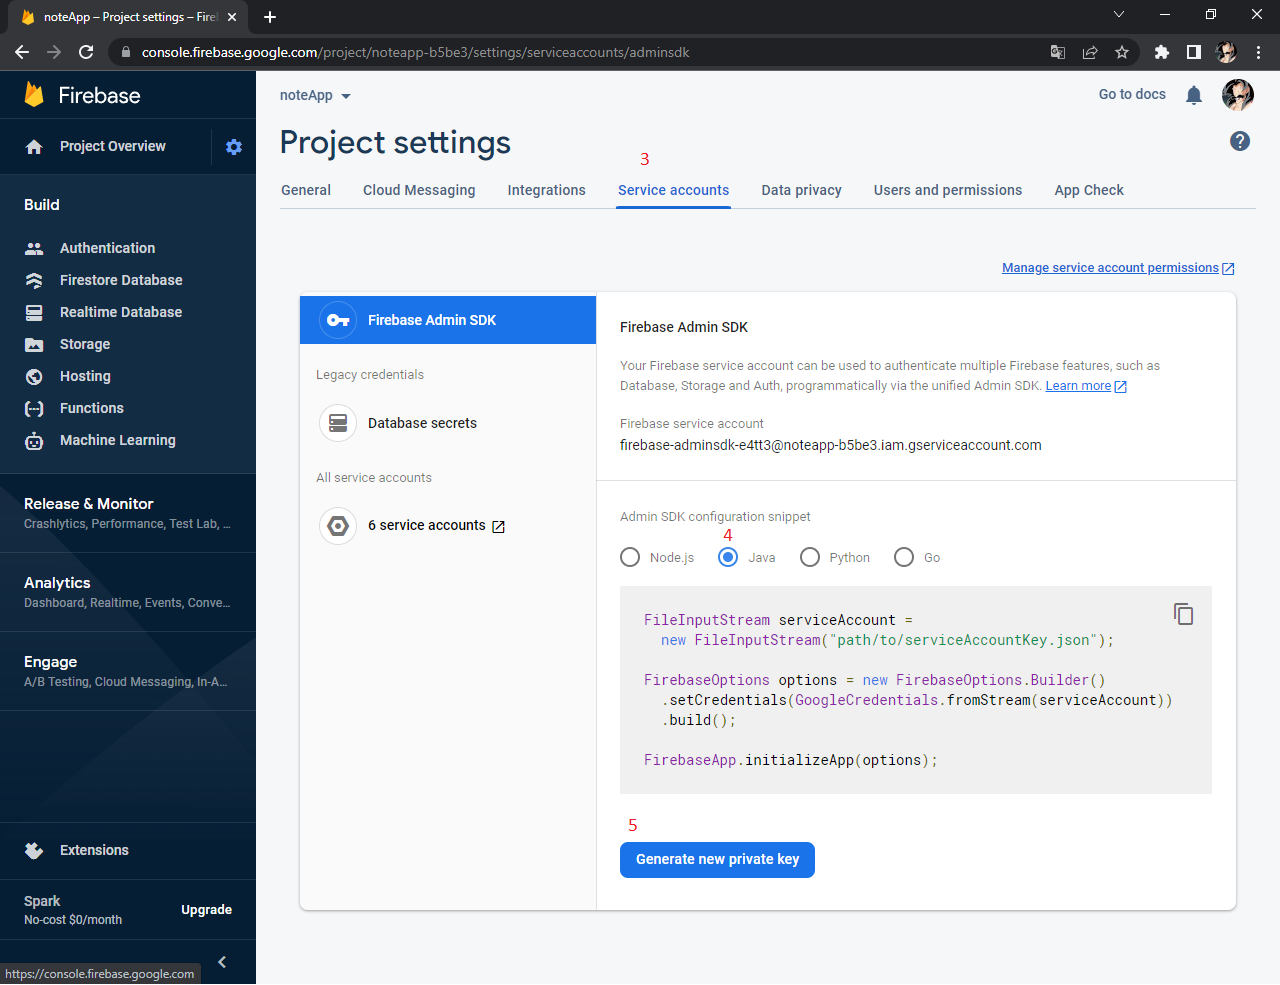
\includegraphics[scale=0.2]{images/config_5.png}
	\caption{Firebase service key generálás}
	\label{fig:firebase_service_key}
\end{figure}
\noindent Nyomjuk meg sorrendben a \ref{fig:firebase_service_key}. ábrán piros számokkal jelölt gombokat, majd a felugró ablaknál a 'Generate key' gombot. Sikeresen letöltöttük a szükséges Firebase Service Key json fájlt!
\vspace{5pt}\\A config.xml fájlban a <dbJsonPath>...</dbJsonPath> tag-ek közé másoljuk be a letöltött json fájl elérési útvonalát. Ezt a leírás elején található példa elérési úthoz hasonlóan tegyük.
\vspace{5pt}\\ Ha lépésről lépésre mindent megtettünk, a config.xml fájl tartalma hasonlóan kell, hogy kinézzen, mint a \ref{fig:config_file_final}. ábrán látható.
\begin{figure}[h]
	\centering
	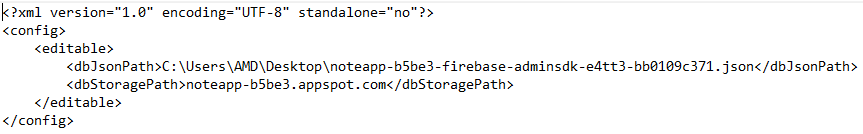
\includegraphics[scale=0.5]{images/config_6.png}
	\caption{Korrekt config.xml felépítés}
	\label{fig:config_file_final}
\end{figure}
\newline
\noindent Végezetül mentsük el, majd zárjuk be a config.xml fájlt, ezután futtassuk a .jar fájlt. Ha hibaüzenetet kapunk vizsgáljuk meg a config.xml fájlt. Nézzük meg, hogy helyesen írtuk-e be az elérési útvonalakat, '\textbackslash' jeleket alkalmaztunk-e a megadásukhoz. \\Ha továbbra is hibaüzenetet kapunk ismételjük el elejéről a lépéseket.
\vspace{5pt}\\ Ha mindent megfelelően adtunk meg a program elindul.


\subsection{Fontos információk}
\textbf{Nagyon fontos}, hogy a .jks fájlt ne töröljük. Ha mégis letöröljük hibákba fogunk ütközni, az alkalmazás adatai elvesznek és nem tudjuk őket sehogy visszaszerezni.
\vspace{5pt}\\Ha töröltük a KeyStore fájlt, akkor \ref{fig:firebase_storage_default}. ábrán lévő felületen töröljük a Storage-ben lévő, programhoz tartozó összes fájlt (appKeyStore.jks, applicationData.xml). Így az előzőleg elmentett titkosított adatok is eltűnnek, és a .jks fájl is. A program ebben az esetben következő futtatáskor új fájlokat generál és üres tartalommal indul.
\vspace{5pt}\\A program futtatásához java futtató környezet szükséges, ezt JRE-nek hívják (Java Runtime Environment). Telepíthetjük az Oracle-féle implementációt is, ami a \\ \href{https://java.com/en/download/manual.jsp}{https://java.com/en/download/manual.jsp} linken érhető el.

\vspace{30pt}\Section{Jegyzetek menü}

Az \ref{fig:menu_notes_2}. ábrán látható a jegyzetek menü felépítése, a pirossal számozott elemek leírása található a kép alatt.

\begin{figure}[h]
	\centering
	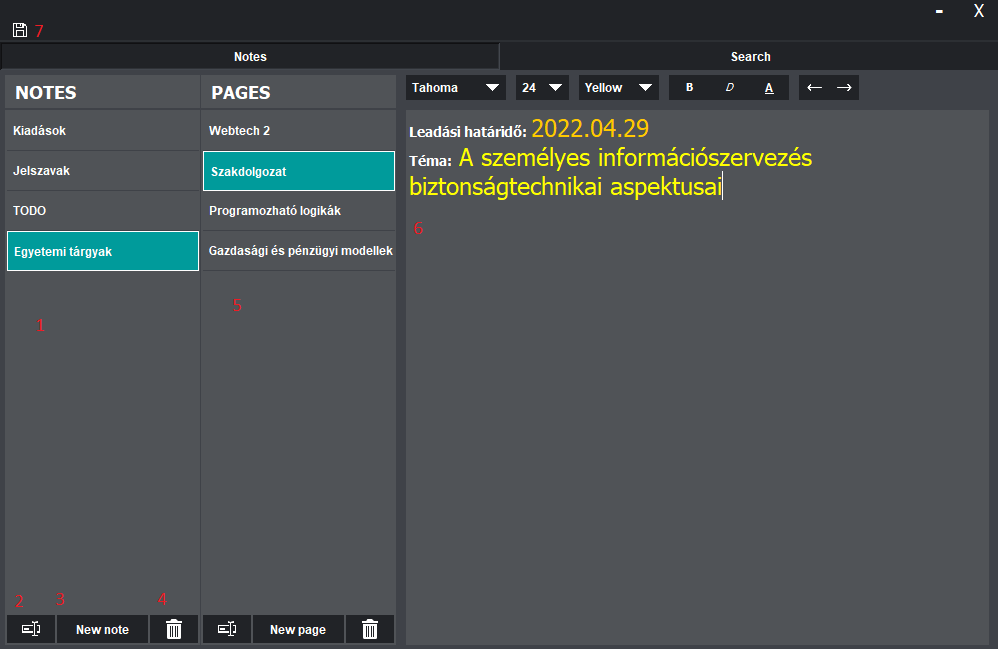
\includegraphics[scale=0.5]{images/doc_1.png}
	\caption{Jegyzetek menü használat közben.}
	\label{fig:menu_notes_2}
\end{figure}

\vspace{5pt} \noindent \textbf{1}-es panel a jegyzetek panelje, itt találhatóak egymás alá beszúrva a különböző jegyzetek. Az éppen kijelölt jegyzet kék színű, kattintással tudunk új jegyzetet kiválasztani, valamint ha a panelen belül az üres részre kattintunk, akkor mindig az utolsó jegyzetet fogja kijelölni.
\newline \\ Található a panelen 3 gomb. 
\vspace{5pt} \\ \textbf{2}-es gomb az éppen kijelölt jegyzet átnevezésére szolgál, egy felugró modális ablakba a beírt szövegre nevezhetjük át a kijelölt elemet, vagy megszakíthatjuk az egész folyamatot. (lásd \ref{fig:menu_notes_rename}. ábra)

\begin{figure}[h]
	\centering
	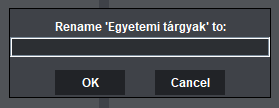
\includegraphics[scale=0.6]{images/doc_2.png}
	\caption{Átnevezésre szolgáló modális ablak.}
	\label{fig:menu_notes_rename}
\end{figure}

\vspace{5pt} \noindent \textbf{3}-mas gombbal új jegyzetet adunk a meglévő jegyzet listához. Alapértelmezett neve a jegyzeteknek ’New Note [sorszám]’. A sorszám a jegyzet id-jével egyezik, nem a listabeli pozíciójával.
\vspace{5pt} \\ \textbf{4}-es gombbal az éppen kijelölt jegyzetet törölhetjük, vagy szakíthatjuk meg ezt a folyamatot egy felugró modális ablak segítségével. (lásd \ref{fig:menu_notes_delete}. ábra)

\begin{figure}[h]
	\centering
	
\includegraphics[scale=0.6]{images/doc_3.png}
	\caption{Törlésre szolgáló modális ablak.}
	\label{fig:menu_notes_delete}
\end{figure}

\vspace{5pt} \noindent \textbf{5}-ös panel a lapok panelje. Minden jegyzetnek külön lapjai lehetnek. A panel egyéb funkciói és kezelése teljesen megegyezik az előbb bemutatott jegyzetek menüével.
\vspace{5pt} \\ Ahogy kattintással váltogatunk a jegyzetek között, úgy frissül a lapok menü is, tehát ahogy a beszúrt képen látszik, az ’Egyetemi tárgyak’ jegyzetnek 4 lapja van. Ha átkattintanánk a ’TODO’-ra, akkor ebben a jegyzetben található lapok listája jelenne meg. Alapvetően jegyzet váltáskor nem jelölődik ki egy lap sem. 
\vspace{10pt} \\ \textbf{6}-os szövegdoboz felületen az éppen kijelölt lap tartalma jelenik meg. A felület mindig frissül, ha új lapra kattintunk, valamint ha nincs egy lap sem kijelölve, akkor üres lesz.
\\A szövegdoboz felett gombok találhatók, amik a szöveg szerkesztésére használhatóak.
\\Balról  jobbra haladva a gombok: 
\vspace{5pt} \\-Szöveg stílus váltás: alapértelmezett Tahoma. Csak a kijelölt szövegrész stílusa fog megváltozni!
\vspace{5pt} \\-Szöveg méret váltás: alapértelmezett 14-as méret. Csak a kijelölt szövegrész mérete fog megváltozni!
\vspace{5pt} \\-Szöveg szín váltás: alapértelmezett fehér szín. Csak a kijelölt szövegrész színe fog megváltozni!
\vspace{5pt} \\-Félkövér betű: kijelölt szövegrész félkövérré alakítása.
\\Gyorsbillentyű: Ctrl + B
\vspace{5pt} \\-Dőlt betű: kijelölt szövegrész dőltté változtatása.
\\Gyorsbillentyű: Ctrl + I
\vspace{5pt} \\-Aláhúzás: kijelölt szövegrész aláhúzása.
\\Gyorsbillentyű: Ctrl + U
\vspace{5pt} \\-Undo gomb: A szövegdoboz utolsó változtatását visszavonja. Fontos, hogy csak a szövegdobozon működik, note vagy page törlésre, átnevezésre, stb… nem!
\\Gyorsbillentyű: Ctrl + Z
\vspace{5pt} \\-Redo gomb: Az undo gomb ellentéte. Fontos, hogy csak a szövegdobozon működik, note vagy page törlésre, átnevezésre, stb… nem!
\\Gyorsbillentyű: Ctrl + Y

\vspace{5pt} \noindent \textbf{7}-essel jelzett gomb a mentés gomb. Gyorsbillentyű: Ctrl + S. Az alkalmazás tartalmát titkosítja majd elmenti az adatbázisba.
\\A gomb megnyomásakor vagy gyorsbillentyű használatakor az alkalmazás kis időre megfagyhat.




\vspace{30pt}\Section{Kereső menü}

Az \ref{fig:menu_search_2}. ábrán látható a kereső menü felépítése, a pirossal számozott elemek leírása található a kép alatt.

\begin{figure}[h]
	\centering
	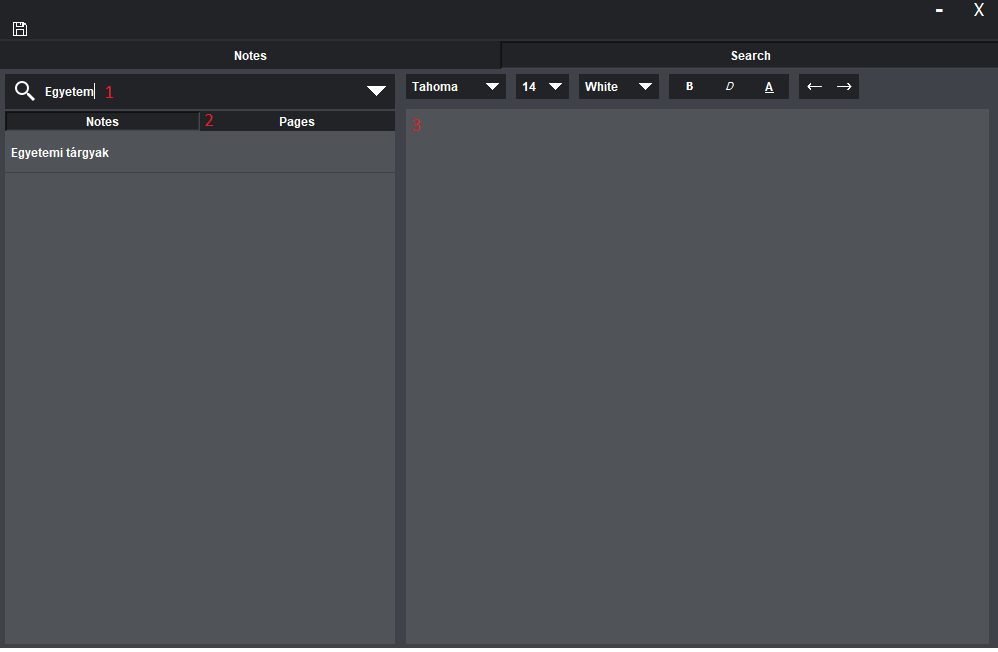
\includegraphics[scale=0.5]{images/doc_4.png}
	\caption{Kereső menü működés közben.}
	\label{fig:menu_search_2}
\end{figure}

\vspace{5pt} \noindent \textbf{1}-essel jelölt elem a ’search bar’ (kereső sor). Jegyzetek, lapok és lapok tartalma között keres. Ha jegyzet neve, lap neve, vagy lap tartalma tartalmazza a beírt kifejezést, akkor lesz találat. 
\vspace{5pt} \\Hogy a keresés könnyebb legyen, üres search bar-ba való kattintáskor az összes jegyzet és lap neve megjelenik egy listába. Ahogy a keresendő szöveget írjuk be a lista annak megfelelően fog változni (lásd \ref{fig:menu_search_searchBar}. ábra). 

\begin{figure}[h]
	\centering
	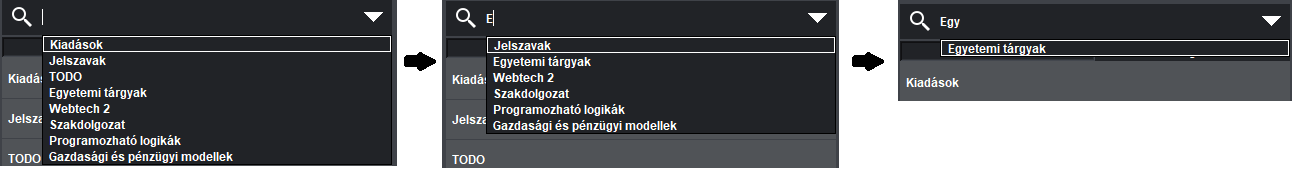
\includegraphics[scale=0.4]{images/doc_5.png}
	\caption{Keresési folyamat szemléltetése.}
	\label{fig:menu_search_searchBar}
\end{figure}
	
\vspace{5pt} \noindent Ha nincs egyezés, a lista eltűnik, nem jelenít meg egyetlen elemet sem.
\vspace{5pt} \\Ha az egyező szöveg egy adott lap tartalmán belül található, tehát nem a nevében, akkor is a listában a lap neve fog szerepelni.
\vspace{5pt} \\A beírt szövegre keresni kijelölés után a nagyítóra való kattintással vagy enter megnyomásával lehetséges.
	
	
\vspace{10pt} \noindent \textbf{2}-essel jelölt elem a Note és Page keresési találatok listája.
\vspace{5pt} \\Alapvetően, ha futtatáskor először lépünk be ebbe a menübe egyik sem lesz kijelölve, viszont az első keresés után a jegyzetek listáját fogja megjeleníteni. Hogyha a page-re kattintunk, akkor a talált lapokat fogja megjeleníteni, így tudunk váltani a talált jegyzetek és lapok, illetve lapok tartalma között.
\vspace{5pt} \\Ha a jegyzet találatok között az egyikre rákattintunk, akkor visszakerülünk a Notes Menu-be, hogy meg tudjuk tekinteni az adott jegyzet lapjait, átnevezni vagy törölni tudjunk.
\vspace{5pt} \\Ha a lap találatok között az egyikre kattintunk, akkor nem kerülünk vissza a Notes Menu-be. Az adott lap tartalmát tudjuk szerkeszteni és megtekinteni egy Notes Menu-höz hasonló szövegdobozban \textbf{(3.elem)}. Ennek funkciói teljesen megegyeznek az említett szövegdobozéval és menteni is a ctrl+s-el kell a változtatásokat, vagy a mentés ikonra kattintva.
\vspace{5pt} \\Ha esetleg átnevezni vagy törölni szeretnénk az adott lapot, a Notes Menu-ben tehetjük ezt meg.

\Section{Ismert bug-ok}
Jelenleg kettő kisebb bug-ról tudok, ami biztosan megtalálható az alkalmazásban. Egyik bug sem 'töri meg' az alkalmazást, de a gördülékeny működéshez jó lenne a közeljövőben megoldani őket.
\\ Mind a felhasználói felülethez köthető, azon belül is a kereső menühöz.
\begin{itemize}
	\item Bármit írunk be a keresőbe, ha több mint egy találatot dob ki, és rányomunk az első lehetőségre, akkor az a keresősáv szövegdobozába mindig a 'New Note 0'-t fogja behelyettesíteni (a jegyzetek listájának első elemének nevét). Ez egyetlen egyező találat esetén nem érvényes.
	\item A másik keresősáv bug pedig ehhez, egyetlen egyezés esetéhez köthető. Tegyük fel rákeresünk a 'New Note 0'-ra, akkor a legördülő menü eltűnik, attól függetlenül, hogy van egyező találat. A szövegdobozra való újabb kattintással jelenik meg. Ha viszont nem teljes egyezőséggel keresünk rá valamire, például azt írjuk be, hogy 'New note 0', akkor megjelenik az egyező találat egyetlen egyezés esetén is.
\end{itemize}
\noindent Szóba kerültek az 5.5. és 5.6. alfejezetben a felhasználói felület létrehozásával kapcsolatos nehézségek, a keresősáv bug-jait is ilyen nehézségek közé sorolnám.
\\Úgy gondolom, ha nem Swing-et, hanem egy modernebb GUI fejlesztő függvény könyvtárat használtam volna, akkor nem találkoztam volna ezekkel a hibákkal.
	\Chapter{Összefoglalás}

Hasonló szerepe van, mint a bevezetésnek.
Itt már múltidőben lehet beszélni.
A szerző saját meglátása szerint kell összegezni és értékelni a dolgozat fontosabb eredményeit.
Meg lehet benne említeni, hogy mi az ami jobban, mi az ami kevésbé jobban sikerült a tervezettnél.
El lehet benne mondani, hogy milyen további tervek, fejlesztési lehetőségek vannak még a témával kapcsolatban.

	\appendix
	\Chapter{Táblázatok}

\begin{table}[H]
	\centering
	\caption{1MB-hoz tartozó titkosítási mérések}
	\label{tab:enc_1mb}
	\medskip
	\begin{tabular}{|p{2.4cm}|p{2cm}|p{2cm}|p{2cm}|p{2cm}|}
		\hline
		\textbf{Titkosítás} \newline \textbf{1MB} & \textbf{AES} & \textbf{DES} & \textbf{Triple DES} & \textbf{Blowfish}\\
		\hline
		\textbf{1.mérés} & 55 & 70 & 105 & 60\\
		\hline
		\textbf{2.mérés} & 51 & 63 & 98 & 65\\
		\hline
		\textbf{3.mérés} & 57 & 68 & 109 & 57\\
		\hline
		\textbf{4.mérés} & 58 & 67 & 102 & 58\\
		\hline
		\textbf{5.mérés} & 55 & 68 & 110 & 62\\
		\hline
		\textbf{6.mérés} & 54 & 71 & 106 & 58\\
		\hline
		\textbf{7.mérés} & 53 & 63 & 102 & 59\\
		\hline
		\textbf{8.mérés} & 57 & 65 & 105 & 64\\
		\hline
		\textbf{9.mérés} & 51 & 70 & 107 & 53\\
		\hline
		\textbf{10.mérés} & 51 & 72 & 100 & 56\\
		\hline
		\hline
		\textbf{Átlag} & \textbf{54,2} & \textbf{67,7} &\textbf{ 104,4} & \textbf{59,2}\\
		\hline
	\end{tabular}
\end{table}

\begin{table}[H]
	\centering
	\caption{1MB-hoz tartozó visszafejtési mérések}
	\label{tab:dec_1mb}
	\medskip
	\begin{tabular}{|p{2.4cm}|p{2cm}|p{2cm}|p{2cm}|p{2cm}|}
		\hline
		\textbf{Visszafejtés} \newline \textbf{1MB} & \textbf{AES} & \textbf{DES} & \textbf{Triple DES} & \textbf{Blowfish}\\
		\hline
		\textbf{1.mérés} & 13 & 29 & 59 & 18\\
		\hline
		\textbf{2.mérés} & 12 & 30 & 58 & 21\\
		\hline
		\textbf{3.mérés} & 11 & 30 & 68 & 18\\
		\hline
		\textbf{4.mérés} & 12 & 31 & 58 & 19\\
		\hline
		\textbf{5.mérés} & 12 & 30 & 59 & 21\\
		\hline
		\textbf{6.mérés} & 12 & 31 & 58 & 18\\
		\hline
		\textbf{7.mérés} & 12 & 32 & 59 & 20\\
		\hline
		\textbf{8.mérés} & 11 & 29 & 59 & 20\\
		\hline
		\textbf{9.mérés} & 12 & 27 & 59 & 18\\
		\hline
		\textbf{10.mérés} & 13 & 30 & 56 & 19\\
		\hline
		\hline
		\textbf{Átlag} & \textbf{12} & \textbf{29,9} & \textbf{59,3} & \textbf{19,2}\\
		\hline
	\end{tabular}
\end{table}

\begin{table}[H]
	\centering
	\caption{2MB-hoz tartozó titkosítási mérések}
	\label{tab:enc_2mb}
	\medskip
	\begin{tabular}{|p{2.4cm}|p{2cm}|p{2cm}|p{2cm}|p{2cm}|}
		\hline
		\textbf{Titkosítás} \newline \textbf{2MB} & \textbf{AES} & \textbf{DES} & \textbf{Triple DES} & \textbf{Blowfish}\\
		\hline
		\textbf{1.mérés} & 52 & 86 & 149 & 71\\
		\hline
		\textbf{2.mérés} & 58 & 85 & 148 & 68\\
		\hline
		\textbf{3.mérés} & 51 & 90 & 157 & 65\\
		\hline
		\textbf{4.mérés} & 56 & 86 & 149 & 66\\
		\hline
		\textbf{5.mérés} & 51 & 85 & 145 & 71\\
		\hline
		\textbf{6.mérés} & 60 & 97 & 161 & 76\\
		\hline
		\textbf{7.mérés} & 55 & 86 & 166 & 69\\
		\hline
		\textbf{8.mérés} & 60 & 95 & 153 & 68\\
		\hline
		\textbf{9.mérés} & 70 & 89 & 157 & 70\\
		\hline
		\textbf{10.mérés} & 54 & 87 & 154 & 74\\
		\hline
		\hline
		\textbf{Átlag} & \textbf{56,7} & \textbf{88,6} & \textbf{153,9} & \textbf{69,8} \\
		\hline
	\end{tabular}
\end{table}

\begin{table}[H]
	\centering
	\caption{2MB-hoz tartozó visszafejtési mérések}
	\label{tab:dec_2mb}
	\medskip
	\begin{tabular}{|p{2.4cm}|p{2cm}|p{2cm}|p{2cm}|p{2cm}|}
		\hline
		\textbf{Visszafejtés} \newline \textbf{2MB} & \textbf{AES} & \textbf{DES} & \textbf{Triple DES} & \textbf{Blowfish}\\
		\hline
		\textbf{1.mérés} & 18 & 48 & 109 & 32\\
		\hline
		\textbf{2.mérés} & 17 & 47 & 110 & 33\\
		\hline
		\textbf{3.mérés} & 17 & 48 & 111 & 32\\
		\hline
		\textbf{4.mérés} & 17 & 48 & 110 & 32\\
		\hline
		\textbf{5.mérés} & 17 & 48 & 110 & 32\\
		\hline
		\textbf{6.mérés} & 20 & 49 & 136 & 33\\
		\hline
		\textbf{7.mérés} & 18 & 49 & 137 & 35\\
		\hline
		\textbf{8.mérés} & 20 & 50 & 111 & 35\\
		\hline
		\textbf{9.mérés} & 18 & 49 & 111 & 32\\
		\hline
		\textbf{10.mérés} & 18 & 50 & 112 & 34\\
		\hline
		\hline
		\textbf{Átlag} & \textbf{18} & \textbf{48,5} & \textbf{115,7} & \textbf{33}\\
		\hline
	\end{tabular}
\end{table}


\begin{table}[H]
	\centering
	\caption{3MB-hoz tartozó titkosítási mérések}
	\label{tab:enc_3mb}
	\medskip
	\begin{tabular}{|p{2.4cm}|p{2cm}|p{2cm}|p{2cm}|p{2cm}|}
		\hline
		\textbf{Titkosítás} \newline \textbf{3MB} & \textbf{AES} & \textbf{DES} & \textbf{Triple DES} & \textbf{Blowfish}\\
		\hline
		\textbf{1.mérés} & 55 & 109 & 205 & 96\\
		\hline
		\textbf{2.mérés} & 64 & 108 & 216 & 80\\
		\hline
		\textbf{3.mérés} & 63 & 114 & 241 & 80\\
		\hline
		\textbf{4.mérés} & 56 & 98 & 209 & 78\\
		\hline
		\textbf{5.mérés} & 60 & 113 & 204 & 84\\
		\hline
		\textbf{6.mérés} & 73 & 117 & 209 & 79\\
		\hline
		\textbf{7.mérés} & 59 & 103 & 238 & 78\\
		\hline
		\textbf{8.mérés} & 64 & 117 & 206 & 81\\
		\hline
		\textbf{9.mérés} & 58 & 113 & 242 & 86\\
		\hline
		\textbf{10.mérés} & 59 & 113 & 204 & 85\\
		\hline
		\hline
		\textbf{Átlag} & \textbf{61,1} & \textbf{110,5} & \textbf{217,4} & \textbf{82,7} \\
		\hline
	\end{tabular}
\end{table}

\begin{table}[H]
	\centering
	\caption{3MB-hoz tartozó visszafejtési mérések}
	\label{tab:dec_3mb}
	\medskip
	\begin{tabular}{|p{2.4cm}|p{2cm}|p{2cm}|p{2cm}|p{2cm}|}
		\hline
		\textbf{Visszafejtés} \newline \textbf{3MB} & \textbf{AES} & \textbf{DES} & \textbf{Triple DES} & \textbf{Blowfish}\\
		\hline
		\textbf{1.mérés} & 20 & 68 & 162 & 41\\
		\hline
		\textbf{2.mérés} & 22 & 67 & 163 & 41\\
		\hline
		\textbf{3.mérés} & 21 & 67 & 199 & 42\\
		\hline
		\textbf{4.mérés} & 21 & 68 & 163 & 42\\
		\hline
		\textbf{5.mérés} & 21 & 69 & 162 & 41\\
		\hline
		\textbf{6.mérés} & 23 & 67 & 164 & 45\\
		\hline
		\textbf{7.mérés} & 21 & 68 & 201 & 42\\
		\hline
		\textbf{8.mérés} & 20 & 67 & 162 & 43\\
		\hline
		\textbf{9.mérés} & 22 & 70 & 200 & 42\\
		\hline
		\textbf{10.mérés} & 21 & 68 & 164 & 45\\
		\hline
		\hline
		\textbf{Átlag} & \textbf{21,2} & \textbf{67,9} & \textbf{174} & \textbf{42,4}\\
		\hline
	\end{tabular}
\end{table}

\begin{table}[H]
	\centering
	\caption{4MB-hoz tartozó titkosítási mérések}
	\label{tab:enc_4mb}
	\medskip
	\begin{tabular}{|p{2.4cm}|p{2cm}|p{2cm}|p{2cm}|p{2cm}|}
		\hline
		\textbf{Titkosítás} \newline \textbf{4MB} & \textbf{AES} & \textbf{DES} & \textbf{Triple DES} & \textbf{Blowfish}\\
		\hline
		\textbf{1.mérés} & 66 & 135 & 258 & 93\\
		\hline
		\textbf{2.mérés} & 63 & 115 & 254 & 95\\
		\hline
		\textbf{3.mérés} & 60 & 137 & 258 & 96\\
		\hline
		\textbf{4.mérés} & 56 & 135 & 255 & 93\\
		\hline
		\textbf{5.mérés} & 58 & 131 & 303 & 94\\
		\hline
		\textbf{6.mérés} & 72 & 137 & 262 & 91\\
		\hline
		\textbf{7.mérés} & 62 & 133 & 263 & 91\\
		\hline
		\textbf{8.mérés} & 66 & 137 & 310 & 95\\
		\hline
		\textbf{9.mérés} & 67 & 123 & 259 & 97\\
		\hline
		\textbf{10.mérés} & 62 & 137 & 270 & 92\\
		\hline
		\hline
		\textbf{Átlag} & \textbf{63,2} & \textbf{132} & \textbf{269,2} & \textbf{93,7}\\
		\hline
	\end{tabular}
\end{table}

\begin{table}[H]
	\centering
	\caption{4MB-hoz tartozó visszafejtési mérések}
	\label{tab:dec_4mb}
	\medskip
	\begin{tabular}{|p{2.4cm}|p{2cm}|p{2cm}|p{2cm}|p{2cm}|}
		\hline
		\textbf{Visszafejtés} \newline \textbf{4MB} & \textbf{AES} & \textbf{DES} & \textbf{Triple DES} & \textbf{Blowfish}\\
		\hline
		\textbf{1.mérés} & 23 & 84 & 212 & 51\\
		\hline
		\textbf{2.mérés} & 23 & 85 & 213 & 53\\
		\hline
		\textbf{3.mérés} & 22 & 83 & 213 & 52\\
		\hline
		\textbf{4.mérés} & 23 & 83 & 213 & 50\\
		\hline
		\textbf{5.mérés} & 22 & 83 & 262 & 40\\
		\hline
		\textbf{6.mérés} & 24 & 91 & 217 & 54\\
		\hline
		\textbf{7.mérés} & 24 & 84 & 216 & 52\\
		\hline
		\textbf{8.mérés} & 23 & 86 & 265 & 52\\
		\hline
		\textbf{9.mérés} & 23 & 88 & 214 & 51\\
		\hline
		\textbf{10.mérés} & 23 & 83 & 266 & 52\\
		\hline
		\hline
		\textbf{Átlag} & \textbf{23} & \textbf{85} & \textbf{229,1} & \textbf{50,7}\\
		\hline
	\end{tabular}
\end{table}
	
	\clearpage
	
	\addcontentsline{toc}{chapter}{Irodalomjegyzék}
	\bibliographystyle{plain}
	\bibliography{dolgozat.bib}
	
	\newpage
	
	
\pagestyle{empty}

\noindent \textbf{\Large CD Használati útmutató}

\vskip 1cm

\noindent A CD 2 fő jegyzéket tartalmaz, az Alkalmazás és a Dokumentumok jegyzéket.
\vspace{5pt} \\Az Alkalmazás mappában megtalálható a
\begin{itemize}
	\item User\_manual mappa, amiben az alkalmazás kezeléséhez szükséges használati útmutató pdf-je található.
	\item Source\_code mappa, ami az elkészített alkalmazás forráskódját tartalmazza. A mappán belül a src/Main/MainClass.java fájlban található az alkalmazást indító main függvény. 
	\\Az elkészített programok telepítéséhez, futtatásához tartozó feltételek a használati útmutatóban vannak leírva. 
	\item Release mappa, melyben az alkalmazás található futtatható .jar kiterjesztésben.
\end{itemize}
\vspace{5pt} A Dokumentumok mappában megtalálható(k) a
\begin{itemize}
	\item Adatszerkezetek, Tervezés és Titkosítási\_dokumentumok mappák, amelyek az összes, a dolgozattal kapcsolatosan összegyűjtött anyagot tartalmazzák .docx, .pdf és .txt kiterjesztésű fájlokban.
	\item CD\_User\_Manual mappa, a CD használati útmutatójának pdf-ét tartalmazza.
	\item Szakdolgozat mappa, amiben a dolgozat LaTeX forráskódja található.
	\item Szakdolgozat\_pdf mappa, ami a szakdolgozat pdf verzióját tartalmazza.
\end{itemize}


	
\end{document}